\chapter{Index Notation and Introduction to Tensors}
\label{chapter:Tensor}

This is the final chapter of this book. (Congratulations!) It will be revealed that, matrices (or to be accurate, linear transformations), along with vectors, actually can be generalized to a broader class of objects known as \textit{tensors}. In the simplest sense, tensors are quantities with subscripts. To facilitate the manipulation of these subscripts, we will introduce the handy \textit{Index Notation}, as well as the \textit{Kronecker delta/epsilon symbols}. The next step is to develop \textit{matrix/tensor calculus} where several important differentiation rules and integral theorems will be given. Tensors can have physical meanings, allowing us to apply them in many scenarios. One of their usages in Earth Science is to serve as the language in \textit{Continuum Mechanics}. On the other hand, the related matrix calculus is much needed in \textit{Data Assimilation}, which is a technique in Atmospheric Sciences to rectify the output of a forecast from a weather model with available observations.

\section{Index Notation and Tensors}

\subsection{Rules of Index Notation}

Previously, we have usually been writing matrix multiplications along the lines of $AB = C$ or $A\vec{x} = \smash{\vec{h}}$ without explicitly showing the subscripts and summation symbol. However, if we choose to do so, then they can be expressed as
\begin{align*}
\sum_{k=1}^r A_{ik}B_{kj} &= C_{ij} &  & \sum_{j=1}^n A_{ij}x_j = h_i
\end{align*}
However, the summation symbol is clumsy to be included every time, especially when it involves a chain of products like $ABCD$. The \index{Index Notation}\keywordhl{Index Notation} (also known as the \index{Einstein Convention}\keywordhl{Einstein Convention}) solves this problem by assuming that any subscript appearing exactly twice in an additive term will be summed (\textit{contracted}) implicitly over all values that the subscript can take. This also means that any such pair of repeated subscripts must
occur only in positions with the same range of values. Consequentially, the above examples are simplified into
\begin{align*}
A_{ik}B_{kj} &= C_{ij} &  & A_{ij}x_j = h_i    
\end{align*}
To be more clear, subscripts that appear exactly twice in any additive term are called \index{Summation Indices}\keywordhl{summation indices} (or \index{Dummy Indices}\keywordhl{dummy indices}) and are summed over specific values which are often automatically inferred from the situation (for example, in three-dimensional physical problems, they will usually take the explicit values of $1,2,3$.). On the other hand, subscripts that only appear once in \textit{every} additive term of an expression or equation are known as \index{Free Indices}\keywordhl{free indices}. In the first example above, $k$ is the dummy index, while $i, j$ are free indices. (How about the second example?\footnote{$j$ is the dummy index and $i$ is the free index.}) There are some other important points about the Index Notation to be emphasized: First, it is not allowed for a subscript to appear more than twice within a single additive term (so we cannot write $A_{ik}B_{kj}C_{kl}$, although it is okay for a dummy subscript to appear twice in multiple additive terms, e.g. $A_{ik}B_{kj} + C_{ij}D_{kk}$); Second, any pair of dummy indices can be replaced by any other alphabets (e.g. $A_{ik}B_{kj}$ is equivalent to $A_{il}B_{lj}$) but the free indices cannot be changed arbitrarily; Finally, as just mentioned, all free indices have to appear once and only once in every additive term (on both sides if it is an equation) (so $A_i + B_{ij}C_{j} + D_{ikk}$ is acceptable but not $A_{ij} + B_{kkj}$). As long as the quantities have their subscripts written out, the order of the quantities (but not their indices) is unimportant. Below we give some examples of the Index Notation in a three-dimensional setting:
\begin{enumerate}
    \item $a_ib_i = \sum_{i=1}^3 a_ib_i = a_1b_1 + a_2b_2 + a_3b_3$
    \item $A_{kk} = \sum_{k=1}^3 A_{kk} = A_{11} + A_{22} + A_{33}$
    \item $A_{ik}B_{jk} = \sum_{k=1}^3 A_{ik}B_{jk} = A_{i1}B_{j1} + A_{i2}B_{j2} + A_{i3}B_{j3}$
    \item \begin{align*}
    A_{ijk}B_{jl}C_{km} &= \sum_{j=1}^3 \sum_{k=1}^3 A_{ijk}B_{jl}C_{km} \\
    &= A_{i11}B_{1l}C_{1m} + A_{i12}B_{1l}C_{2m} + A_{i13}B_{1l}C_{3m} \\
    &\quad + A_{i21}B_{2l}C_{1m} + A_{i22}B_{2l}C_{2m} + A_{i23}B_{2l}C_{3m} \\
    &\quad + A_{i31}B_{3l}C_{1m} + A_{i32}B_{3l}C_{2m} + A_{i33}B_{3l}C_{3m} \\
    &\coloneq Y_{ilm}
    \end{align*}
    will be a subscripted quantity with 3 free indices $i, l, m$ where each additive term contains $3^2 = 9$ smaller terms.
    \item \begin{align*}
    A_{ikl}B_{jkm}C_{lm} &= \sum_{k=1}^3 \sum_{l=1}^3 \sum_{m=1}^3 A_{ikl}B_{jkm}C_{lm} \\
    &\coloneq Z_{ij}
    \end{align*}
    will be a subscripted quantity with 2 free indices $i, j$ where each additive term contains $3^3 = 27$ smaller terms.
    \item $A_{ij}B_{ijkl}C_{kl} = \smash{\sum_{i=1}^3 \sum_{j=1}^3 \sum_{k=1}^3 \sum_{l=1}^3} A_{ij}B_{ijkl}C_{kl} \coloneq X$ will be a scalar quantity without free indices consisting of $3^4 = 81$ smaller terms.
\end{enumerate}
Short Exercise: Determine whether the following equations are valid or not, and justify your answers.\footnote{Incorrect ($j$ appears three times in the single additive term on R.H.S.), Correct ($i,j$ are free indices and $k,l$ are dummy indices), Incorrect ($j$ appears twice on L.H.S. but once on R.H.S), Correct (All subscripts are dummy indices and all additive terms are scalars), Incorrect ($i,j$ cannot be free and dummy indices at the same time).}
\begin{enumerate}
    \item $x_i = u_jv_{ijj}$;
    \item $A_{ij} = B_{ik}C_{kj} + D_{jl}x_iy_l$;
    \item $A_{ij}x_j = B_{ij}$;
    \item $A_{ii} + u_jv_j = B_{kl}C_{km}w_{lm} - 1$;
    \item $A_{ij} + B_{ij}C_{ij} = D_{ij}$.
\end{enumerate}

\subsection{Kronecker Delta and Epsilon Symbols}

Before getting to know about the \textit{Kronecker delta/epsilon symbols}, it is helpful to denote the three-dimensional Cartesian standard unit vectors $\hat{\imath} = \hat{e}^{(1)}$, $\hat{\jmath} = \hat{e}^{(2)}$, $\hat{k} = \hat{e}^{(3)}$ by $\textbf{e}_1, \textbf{e}_2, \textbf{e}_3$ to switch and ensure the consistency of notation. We will assume that the problem is always three-dimensional so that every index always runs through $1,2,3$ unless otherwise specified. Therefore, given any three-dimensional vector $\textbf{u} = (u_1, u_2, u_3)^T$, it can be expressed by 
\begin{align}
\textbf{u} = u_1 \textbf{e}_1 + u_2 \textbf{e}_2 + u_3 \textbf{e}_3 = u_i \textbf{e}_i
\end{align}
using the Index Notation. Now, the \index{Kronecker Delta}\keywordhl{Kronecker delta} symbol is defined as
\begin{defn}[Kronecker Delta Symbol]
The Kronecker delta symbol is a quantity with $2$ subscripts such that
\begin{align}
\delta_{ij} = \begin{cases}
1 & \text{if $i=j$} \\
0 & \text{if $i\neq j$}
\end{cases}    
\label{eqn:krondef}
\end{align}
\end{defn}
Compared with Definition \ref{defn:identity}, it works like and can be treated as an identity matrix, although there are some subtle differences between them. Due to the definition of the delta symbol, its effect is to replace a dummy index with the other index. For example,
\begin{align*}
A_{ij}\delta_{jk} &= A_{ik} & & A_{ij}B_{kl}\delta_{jl} = A_{ij}B_{kj}
\end{align*}
since only when $j = k$ the delta symbol will be equal to $1$ and otherwise $0$ in the first case (how about the second case?). Recall that for the standard unit vectors, we have
\begin{subequations}
\begin{align}
\textbf{e}_1 \cdot \textbf{e}_1 = \textbf{e}_2 \cdot \textbf{e}_2 = \textbf{e}_3 \cdot \textbf{e}_3 &= 1 \\
\textbf{e}_1 \cdot \textbf{e}_2 = \textbf{e}_1 \cdot \textbf{e}_3 = \textbf{e}_2 \cdot \textbf{e}_3 &= 0
\end{align}
\end{subequations}
or more succinctly,
\begin{align}
\textbf{e}_i \cdot \textbf{e}_j = \begin{cases}
1 & \text{if $i=j$} \\
0 & \text{if $i\neq j$}
\end{cases}    
\end{align}
Hence we can define the Kronecker delta symbol via
\begin{align}
\delta_{ij} = \textbf{e}_i \cdot \textbf{e}_j \label{eqn:kronee}
\end{align}
With this, we can derive (\ref{eqn:dotreal}) in Definition \ref{defn:dotreal} for the real dot product in a new way:
\begin{align}
\textbf{u} \cdot \textbf{v} &= (u_i \textbf{e}_i) \cdot (v_j \textbf{e}_j) \nonumber \\
&= u_iv_j (\textbf{e}_i \cdot \textbf{e}_j) \nonumber \\
&= u_iv_j \delta_{ij} & \text{(by (\ref{eqn:kronee}))} \nonumber \\
&= u_iv_i \label{eqn:dotind}
\end{align}
On the other hand, the \index{Epsilon Symbol}\index{Permutation Symbol}\keywordhl{epsilon (permutation)} symbol (or the \index{Levi-Civita Symbol}\keywordhl{Levi-Civita symbol}) is defined as
\begin{defn}[Levi-Civita Epsilon Symbol]
\label{defn:epsilon}
The epsilon permutation symbol is a quantity with $3$ subscripts such that
\begin{align}
\label{eqn:epsilon}
\epsilon_{ijk} =
\begin{cases}
0 & \text{if any two indices are equal} \\
+1 & \begin{aligned}
&\text{if $(i,j,k)$ is an even permutation of $(1,2,3)$,} \\
&\text{i.e.\ $(1,2,3), (2,3,1), (3,1,2)$}
\end{aligned}  \\
-1 & \begin{aligned}
&\text{if $(i,j,k)$ is an odd permutation of $(1,2,3)$,} \\
&\text{i.e.\ $(2,1,3), (3,2,1), (1,3,2)$}
\end{aligned}
\end{cases}    
\end{align}
\end{defn}
Similarly, recall that from Definition \ref{defn:crossijk}, we have
\begin{subequations}
\begin{align}
\textbf{e}_1 \times \textbf{e}_2 &= \textbf{e}_3, \textbf{e}_2 \times \textbf{e}_1 = -\textbf{e}_3 \\
\textbf{e}_2 \times \textbf{e}_3 &= \textbf{e}_1, \textbf{e}_3 \times \textbf{e}_2 = -\textbf{e}_1 \\
\textbf{e}_3 \times \textbf{e}_1 &= \textbf{e}_2, \textbf{e}_1 \times \textbf{e}_3 = -\textbf{e}_2 \\
\textbf{e}_1 \times \textbf{e}_1 &= \textbf{e}_2 \times \textbf{e}_2 = \textbf{e}_3 \times \textbf{e}_3 = \textbf{0}
\end{align}   
\end{subequations}
and thus by going through all the cases, they can be summarized as
\begin{align}
\textbf{e}_i \times \textbf{e}_j= \epsilon_{ijk} \textbf{e}_k \label{eqn:epsilonee}
\end{align}
By taking a dot product with $\textbf{e}_l$ on both sides and adjusting the indices, we can arrive at an equivalent definition of the epsilon symbol:
\begin{align}
\textbf{e}_l \cdot (\textbf{e}_i \times \textbf{e}_j) &= \epsilon_{ijk} (\textbf{e}_l \cdot \textbf{e}_k)  \nonumber \\
\textbf{e}_l \cdot (\textbf{e}_i \times \textbf{e}_j) &= \epsilon_{ijk} \delta_{lk} \nonumber \\
\textbf{e}_l \cdot (\textbf{e}_i \times \textbf{e}_j) &= \epsilon_{ijl} \nonumber \\
\textbf{e}_k \cdot (\textbf{e}_i \times \textbf{e}_j) &= \epsilon_{ijk} \nonumber & \begin{aligned}
&\text{(Replacing a free index $l \to k$} \\
&\text{on both sides simultaneously is allowed)}     
\end{aligned} \\
\epsilon_{jki} &= \textbf{e}_i \cdot (\textbf{e}_j \times \textbf{e}_k) & \text{(Rotating the free indices $k \to i$, $i \to j$, $j \to k$)}  \nonumber \\
\epsilon_{ijk} &= \textbf{e}_i \cdot (\textbf{e}_j \times \textbf{e}_k) 
&\begin{aligned}
&\text{($(j,k,i)$ is an even permutation of $(i,j,k)$} \\
&\text{and can be rotated within the epsilon symbol)}    
\end{aligned} 
\end{align}
In the same spirit, we can derive the formula of cross product in Properties \ref{proper:crossdet} by the Index Notation as follows.
\begin{align}
\textbf{u} \times \textbf{v} &= u_i\textbf{e}_i \times v_j\textbf{e}_j \nonumber \\
&= u_iv_j (\textbf{e}_i \times \textbf{e}_j) \nonumber \\
&= u_iv_j \epsilon_{ijk} \textbf{e}_k \label{eqn:crossind} \\
& \text{(by (\ref{eqn:epsilonee}))} \nonumber \\
&= (u_2v_3 - u_3v_2)\textbf{e}_1 + (u_3v_1 - u_1v_3)\textbf{e}_2 + (u_1v_2 - u_2v_1)\textbf{e}_3 \nonumber \\
& \text{(Direct expansion using (\ref{eqn:epsilon}) in Definition \ref{defn:epsilon})} \nonumber
\end{align}
Comparing with the determinant form of cross product (\ref{eqn:crossdet}) in Properties \ref{proper:crossdet}, we have
\begin{align}
\textbf{u} \times \textbf{v} = u_iv_j \epsilon_{ijk} \textbf{e}_k = 
\begin{vmatrix}
\textbf{e}_1 & \textbf{e}_2 & \textbf{e}_3 \\
u_1 & u_2 & u_3 \\
v_1 & v_2 & v_3
\end{vmatrix}
\label{eqn:crosstens}
\end{align}
Replacing $\textbf{e}_k$ by an arbitrary vector $w_k$, we arrive at an alternative formula for determinant using the Index Notation in three-dimensional vector spaces:
\begin{align}
u_iv_j \epsilon_{ijk} w_k &= 
\begin{vmatrix}
w_1 & w_2 & w_3 \\
u_1 & u_2 & u_3 \\
v_1 & v_2 & v_3
\end{vmatrix}  \nonumber \\
\epsilon_{ijk}  u_iv_jw_k &= 
\begin{vmatrix}
u_1 & u_2 & u_3 \\
v_1 & v_2 & v_3 \\
w_1 & w_2 & w_3
\end{vmatrix} \label{eqn:determinanteps1} \\
& \text{(Swapping rows twice leaves the sign of determinant unchanged)} \nonumber
\end{align}
These two symbols are closely related by the \index{Epsilon-delta Identity}\keywordhl{Epsilon-delta Identity}.
\begin{proper}[$\epsilon$--$\delta$ Identity] 
\label{proper:epsdel} Contracting over the pair of first subscripts between two epsilon symbols gives 
\begin{align}
\epsilon_{ijk}\epsilon_{imn} = \delta_{jm}\delta_{kn} - \delta_{jn}\delta_{km} \label{eqn:epsdel}
\end{align}
\end{proper}
\begin{proof}
We will use a brute-force approach and enumerate all the outcomes. Note that the R.H.S. will have values 
\begin{align}
\begin{cases}
+1 & \text{if $j=m$, $k=n$, $j\neq n$ (and thus $k\neq m$)} \\
-1 & \text{if $j=n$, $k=m$, $j\neq m$ (and thus $k\neq n$)} \\
0 & \text{Otherwise}
\end{cases}
\label{eqn:epsdel2}
\end{align}
Now consider the L.H.S. As the first indices of the two epsilons are equal and every index can only take the three values of $1,2,3$, for their product to give a non-zero value, the only two possibilities are (1) $j = m \neq i$, $k = n \neq i$, $j \neq n$; and (2) $j = n \neq i$, $k = m \neq i$, $j \neq m$ where the four free indices $j,k,m,n$ cannot take the same value as the dummy index $i$, and $j,k$ (also $m,n$) cannot be equal simultaneously. These are consistent with the first and second situations in (\ref{eqn:epsdel2}). Now we only need to justify if they really lead to the outputs of $+1$ and $-1$ respectively. In the first case, it is not hard to see that $\epsilon_{ijk}$ and $\epsilon_{imn}$ must be $+1$ or $-1$ at the same time so their product indeed gives $+1$. Similarly, in the second case, one of the epsilon symbols will be $+1$ and the other will be $-1$ ($\epsilon_{ijk} = -\epsilon_{ikj} = -\epsilon_{imn}$) so it will produce $-1$. The identity is hence established.
\end{proof}
Note that contracting one more index (e.g. $j=m$) in the identity gives
\begin{align}
\epsilon_{ijk}\epsilon_{ijn} &= \delta_{jj}\delta_{kn} - \delta_{jn}\delta_{kj} \nonumber \\
&= 3\delta_{kn} - \delta_{kn} = 2\delta_{kn}
\end{align}
as $\delta_{jj} = \delta_{11} + \delta_{22} + \delta_{33} = 1+1+1 = 3$ and in the second term the dummy index $j$ is replaced by $k$. Going one step further, contracting all three indices simply gives
\begin{align}
\epsilon_{ijk}\epsilon_{ijk} &= 2\delta_{kk} = 2(3) = 6
\end{align}
Now let's see how this identity can be used in showing other vector identities.
\begin{exmp}
Prove Formula (\ref{eqn:triplecross}) for vector triple product in Properties \ref{proper:triplecross} using the Index Notation and Epsilon-delta Identity.
\end{exmp}
\begin{solution}
Applying (\ref{eqn:crossind}) twice, we have
\begin{align*}
\vec{u} \times (\vec{v} \times \vec{w}) &= (u_j\textbf{e}_j) \times (v_mw_n\epsilon_{mni}\textbf{e}_i) \\
&= (u_j\epsilon_{jik}(v_mw_n\epsilon_{mni})) \textbf{e}_k \\
&= \epsilon_{ikj}\epsilon_{imn}u_jv_mw_n \textbf{e}_k \\
&= (\delta_{km}\delta_{jn} - \delta_{kn}\delta_{jm})(u_jv_mw_n \textbf{e}_k) & \text{((\ref{eqn:epsdel}) in Properties \ref{proper:epsdel})} \\
&= u_jv_kw_j \textbf{e}_k - u_jv_jw_k \textbf{e}_k \\
&= (u_jw_j)(v_k\textbf{e}_k) - (u_jv_j)(w_k \textbf{e}_k) \\
&= (\vec{u} \cdot \vec{w})\vec{v} - (\vec{u} \cdot \vec{v})\vec{w} & \text{(by (\ref{eqn:dotind}))}
\end{align*}
\end{solution}
When there is no ambiguity, we will omit the standard unit vector symbol $\textbf{e}_k$ so that, for example, the second-to-last line above is simply $(u_jw_j)v_k - (u_jv_j)w_k$ and a vector $\vec{v}$ is simply denoted by something like $v_i$.

\subsection{Transformation and Quotient Laws for Tensors}

Now we will formally introduce \index{Tensors}\keywordhl{tensors}. A scalar is a rank-$0$ tensor and a vector is a rank-$1$ tensor. The \index{Rank (of a Tensor)}\keywordhl{rank} of a tensor (not to be confused with the rank of a matrix) is the number of its subscripts. Linear transformations or bilinear forms will be rank-$2$ tensors where the associated matrices serve as their representations in certain coordinate systems. Note that this explanation is a largely simplified one and for Mathematicians the definition will be much more rigorous.\footnote{\label{foot:rstensor}Going into depth, the rank of a tensor is actually given by a $2$-tuple $(r,s)$ which means that it receives $r$ \textit{covectors} and $s$ vectors to output a scalar. A covector takes one vector to produce a scalar and hence by definition is a $(0,1)$-tensor, while vice versa a vector will take one covector to also produce a scalar and is a $(1,0)$-tensor. Linear transformations are usually treated as $(1,1)$-tensors while bilinear forms are $(0,2)$-tensors. $r$ and $s$ indicates the number of \textit{contravariant}/\textit{covariant} indices.} But for Physicists or Earth Scientists, it is adequate to know that a rank-$r$ tensor \textit{"transforms like a tensor"}, obeying the so-called \textit{Transformation Law}. To this end, we first need to revisit how a coordinate transformation is carried out. As in (\ref{eqn:PBB'}), the change of coordinates matrix is
\begin{align}
P_\beta^{\beta'} = \begin{bmatrix}
[\vec{v}_\beta^{(1)}]_{\beta'} | [\vec{v}_\beta^{(2)}]_{\beta'} | \cdots | [\vec{v}_\beta^{(n)}]_{\beta'}
\end{bmatrix}
\end{align}
In most of Earth Science usages, the coordinate systems used will be orthonormal and we will assume this is so for the rest of the chapter. This makes the tensors \textit{Cartesian}. By Properties \ref{proper:orthocoords}, the coordinates of any vector in the new orthonormal coordinate system relative to the old orthonormal coordinate system can be found by direct projection and vice versa. Therefore, if we denote the old and new orthonormal basis by $\beta = \{\textbf{e}_1, \textbf{e}_2, \textbf{e}_3\}$ and $\beta'= \{\textbf{e}'_1, \textbf{e}'_2, \textbf{e}'_3\}$, the change of coordinates matrix will become
\begin{align}
P_\beta^{\beta'} = \begin{bmatrix}
\textbf{e}_1 \cdot \textbf{e}'_1 & \textbf{e}_2 \cdot \textbf{e}'_1 & \textbf{e}_3 \cdot \textbf{e}'_1 \\
\textbf{e}_1 \cdot \textbf{e}'_2 & \textbf{e}_2 \cdot \textbf{e}'_2 & \textbf{e}_3 \cdot \textbf{e}'_2 \\
\textbf{e}_1 \cdot \textbf{e}'_3 & \textbf{e}_2 \cdot \textbf{e}'_3 & \textbf{e}_3 \cdot \textbf{e}'_3 
\end{bmatrix}
= \textbf{e}_j \cdot \textbf{e}'_i
\label{eqn:Peeij}
\end{align}
This is an orthogonal matrix\footnote{\label{foot:orthodelta} Extending Properties \ref{proper:orthocoords}, we have $\textbf{e}'_{j} = (\textbf{e}'_{j} \cdot \textbf{e}_{k})\textbf{e}_{k}$ which expresses any new basis vector in terms of the sum of projections onto the old orthonormal basis. By considering $\textbf{e}'_{i} \cdot \textbf{e}'_{j} = \delta_{ij}$ due to (\ref{eqn:kronee}) (valid for any orthonormal basis), we have
\vspace{\maxdimen}
\begin{align*}
(\textbf{e}'_{i} \cdot \textbf{e}_{k})\textbf{e}_{k} \cdot (\textbf{e}'_{j} \cdot \textbf{e}_{l})\textbf{e}_{l} &= \delta_{ij} \\
(\textbf{e}'_{i} \cdot \textbf{e}_{k})(\textbf{e}'_{j} \cdot \textbf{e}_{l})(\textbf{e}_{k} \cdot \textbf{e}_{l}) &= \delta_{ij} \\
(\textbf{e}'_{i} \cdot \textbf{e}_{k})(\textbf{e}'_{j} \cdot \textbf{e}_{l})\delta_{kl} &= \delta_{ij} & \text{($\textbf{e}_{k} \cdot \textbf{e}_{l} = \delta_{kl}$ from (\ref{eqn:kronee}) as well)} \\
(\textbf{e}'_{i} \cdot \textbf{e}_{k})(\textbf{e}'_{j} \cdot \textbf{e}_{k}) &= \delta_{ij}
\end{align*} where the L.H.S. is essentially $(\textbf{e}'_{i} \cdot \textbf{e}_{k})(\textbf{e}_{k} \cdot \textbf{e}'_{j}) = [\smash{(P_\beta^{\beta'})^T}]_{ik}[\smash{P_\beta^{\beta'}}]_{kj}$ and R.H.S. is effectively an identity matrix, so by Properties \ref{proper:orthoinvT} we are done.}, and by (\ref{eqn:bijectvTv}), any vector $\vec{v}$ (that is also a rank-$1$ tensor) is transformed according to
\begin{align}
[\vec{v}]' &= P_\beta^{\beta'}[\vec{v}] \nonumber \\
v'_i &= (\textbf{e}_j \cdot \textbf{e}'_i) v_j \nonumber \\
v'_j &= (\textbf{e}_i \cdot \textbf{e}'_j) v_i 
\end{align}
where we only keep the prime to denote the new coordinate frame as a shorthand and have swapped the indices in the last line. From now on, we will write 
\begin{align}
a_{ij} = \textbf{e}_i \cdot \textbf{e}'_j \label{eqn:aij}
\end{align} for convenience, so the above becomes $v'_j = a_{ij}v_i$. Similarly, for a rank-$2$ tensor $F$, be it a linear transformation or bilinear form, it is transformed as
\begin{align}
F'_{kl} = a_{ik} a_{jl} F_{ij} \label{eqn:rank2aF}
\end{align}
This is consistent with both Properties \ref{proper:endomorph} and Definition \ref{defn:coordtransquad} at the same time, because the change of coordinates matrix is orthogonal and so $[a^{-1}]_{ki} = [a^T]_{ki} = a_{ik}$ by Properties \ref{proper:orthoinvT}. In general, the \keywordhl{Transformation Law} says
\begin{proper}
\label{proper:translaw}
A rank-$r$ \textit{Cartesian} tensor $T$ is a quantity that transforms according to the rule\footnotemark
\begin{align}
T'_{ijkl\ldots} = a_{mi}a_{nj}a_{pk}a_{ql}\cdots T_{mnpq\ldots}
\end{align}
where $a_{**}$ invokes the orthogonal transformation matrix as in (\ref{eqn:aij}).
\end{proper}
\footnotetext{As we are sticking with orthonormal coordinate systems and orthogonal transformations only, the difference between contravariant/covariant indices (as mentioned in Footnote \ref{foot:rstensor}) and hence superscripts/subscripts can be safely ignored for Cartesian tensors. If you don't understand any of what I am saying, ignore this footnote as well.} Physically, it means that tensors are coordinate-independent quantities even though they can have different coordinate representations: These different representations have to be consistent and abide by the Transformation Law so that they still reflect the same physical quantity no matter the choice of coordinate system. Moreover, it implies that to consider if a quantity is a tensor requires a physical context as hinted by the example below.
\begin{exmp}
Show that the following quantities $T = (v_1, v_2) = $ 
\begin{enumerate}[label=(\alph*)]
    \item $(x_2,x_1)$
    \item $(x_1^2,x_1x_2)$
\end{enumerate}
are actually not rank-$1$ Cartesian tensors despite looking like vectors (where the index only takes the values of $1,2$ here).
\end{exmp}
\begin{solution}
For (a), the usual coordinate transformations on $x$ and $y$ respectively by an orthogonal rotation over the plane of a degree $\theta$ are given by (\ref{eqn:2drotate}):
\begin{empheq}[left={\empheqlbrace}]{alignat=1}
x_1' &= (\cos \theta) x_1 + (\sin\theta) x_2 = v_2' \nonumber\\
x_2' &= (-\sin \theta) x_1 + (\cos\theta) x_2 = v_1' \nonumber
\end{empheq}
However, the Transformation Law (Properties \ref{proper:translaw}) requires that
\begin{align*}
v_1' = T'_1 &= a_{11}T_1 + a_{21}T_2 \\
&= (\cos \theta) x_2 + (\sin \theta) x_1 \\
v_2' = T'_2 &= a_{12}T_1 + a_{22}T_2 \\
&= (-\sin\theta) x_2 + (\cos\theta) x_1
\end{align*}
where 
\begin{align*}
a_{ij} &= \textbf{e}_i \cdot \textbf{e}'_j \\
\begin{bmatrix}
a_{11} & a_{12} \\
a_{21} & a_{22}
\end{bmatrix}
&= 
\left[\begin{array}{@{\,}wc{25pt}wc{30pt}@{\,}}
\textbf{e}_1 \cdot \textbf{e}'_1 & \textbf{e}_1 \cdot \textbf{e}'_2 \\
\textbf{e}_2 \cdot \textbf{e}'_1 & \textbf{e}_2 \cdot \textbf{e}'_2
\end{array}\right]
\\
&=
\left[\begin{array}{@{\,}wc{25pt}wc{30pt}@{\,}}
\cos\theta & -\sin\theta \\
\sin\theta & \cos\theta
\end{array}\right]
\end{align*}
These two do not match. For (b), we similarly have
\begin{align*}
v_1' = (x_1')^2 &= ((\cos \theta) x_1 + (\sin\theta) x_2)^2 \\
&= (\cos \theta)^2 x_1^2 + (\cos \theta)(\sin\theta) x_1x_2 + (\sin\theta)^2 x_2^2
\end{align*}
for the first component, but the Transformation Law demands that
\begin{align*}
v_1' = T'_1 = (x_1^2)' &= a_{11}T_1 + a_{21}T_2 \\
&= (\cos \theta) x_1^2 + (\sin \theta) x_1x_2
\end{align*}
They are clearly incompatible. Nevertheless, it is quite easy to see that the intuitive displacement vector $\vec{x} = (x_1,x_2)^T$, as well as $(x_2,-x_1)^T$, will be a rank-$1$ tensor (we leave the verification to the readers\footnote{For the second case $T = (x_2, -x_1)$, the usual coordinate transformation is the essentially same as in part (a) of the example but with an extra negative sign for the second component, whereas the Transformation Law works as
\begin{align*}
v_1' = T'_1 &= a_{11}T_1 + a_{21}T_2 \\
&= (\cos \theta) x_2 + (\sin \theta) (-x_1) \\
&= (\cos \theta) x_2 + (-\sin \theta) x_1 = x_2' \\
v_2' = T'_2 &= a_{12}T_1 + a_{22}T_2 \\
&= (-\sin\theta) x_2 + (\cos\theta) (-x_1) \\
&= -[(\cos \theta) x_2 + (\sin\theta) x_1] = -x_1'
\end{align*} so they are consistent.}).
\end{solution}
It is not hard to show that the product of two tensors is a tensor.\footnote{For example, if $C_{ij\ldots pq\ldots} = A_{ij\ldots}B_{pq\ldots}$ where $A$ and $B$ are tensors, then each of the smaller tensors will transform accordingly on its own: $A'_{mn\ldots} = a_{im}a_{jn}\cdots A_{ij\ldots}$, $B'_{sr\ldots} = a_{ps}a_{qr}\cdots B_{pq\ldots}$, and thus
\begin{align*}
C'_{mn\ldots sr\ldots} = A'_{mn\ldots}B'_{sr\ldots} &= a_{im}a_{jn}\cdots a_{ps}a_{qr}\cdots A_{ij\ldots} B_{pq\ldots} \\
&= a_{im}a_{jn}\cdots a_{ps}a_{qr}\cdots C_{ij\ldots pq\ldots}
\end{align*} will also transform as indicated by Properties \ref{proper:translaw}.} Therefore, kinetic energy (per unit mass) in Newtonian Mechanics $\frac{1}{2}(\vec{v} \cdot \vec{v}) = \frac{1}{2}v_iv_i$ is a rank-$0$ tensor (scalar) if we gladly accept the intuitive premise that the velocity $\vec{v} = v_i$ is a rank-$1$ tensor (vector). In addition, there is another way to quickly verify if a quantity is a tensor by the \keywordhl{Quotient Law} which works in the other way around.
\begin{thm}[Quotient Law]
\label{thm:quotientl}
If $A_{ij\ldots n}$ is a $n$-subscripted quantity, $B_{pq\ldots m}$ is known to be a rank-$m$ tensor, and the product
\begin{align*}
C_{ij\ldots npq \ldots m} = A_{ij\ldots k\ldots n} B_{pq\ldots k\ldots m}   
\end{align*}
is also a tensor of rank $n+m-2k$ where $k \geq 1$ is the amount of index contraction, then $A_{ij\ldots n}$ will be a rank-$n$ tensor.
\end{thm}
With this, we can easily show that some other commonly seen physical quantities are tensors. It will be of use later. 

\subsection{Isotropic Tensors}

Here we will revisit the Kronecker delta and epsilon symbols. In fact, they qualify as a rank-$2$ and rank-$3$ tensor respectively. Moreover, they are further \index{Isotropic}\keywordhl{isotropic} tensors in the sense that they have the same representation (i.e.\ no directionality) in any coordinate system under the Transformation Law. From another perspective, it has to be isotropic since their components are all constants ($0$, $1$, or $-1$) and the usual coordinate transformation should have no effect on them. Now we will explicitly show the isotropic attribute for the Kronecker delta first. The Transformation Law (Properties \ref{proper:translaw}) requires that
\begin{align}
\delta'_{ij} = \delta_{ij}
\end{align}
and the L.H.S. will transform as
\begin{align*}
\delta'_{ij} &= a_{ki}a_{lj}\delta_{kl} \\
&= a_{ki}a_{kj} \\
&= [a^T]_{ik}a_{kj} = \delta_{ij}
\end{align*}
since $a_{**}$ acts as an orthogonal matrix, and by Properties \ref{proper:orthoinvT}, it will equal to R.H.S. which is like an identity (also see Footnote \ref{foot:orthodelta}). This indeed shows that the Kronecker delta is a rank-$2$ isotropic tensor. In a similar vein, we want to show that
\begin{align}
\epsilon'_{ijk} = \epsilon_{ijk}
\end{align}
For this, it is beneficial to first establish that for a $3 \times 3$ matrix $L$, we can extend (\ref{eqn:determinanteps1}) as
\begin{align}
\abs{L}\epsilon_{lmn} = L_{li}L_{mj}L_{nk}\epsilon_{ijk} \label{eqn:determinanteps2}
\end{align}
where $\abs{L}$ is the determinant of $L$. This can be derived by noting that from (\ref{eqn:determinanteps1}) we have
\begin{align}
\abs{L} = L_{1i}L_{2j}L_{3k}\epsilon_{ijk} \label{eqn:determinanteps3}
\end{align}
and swapping or rotating indices, through the properties of the epsilon symbol (or equivalently those of the determinant) will give the other five non-zero possibilities
\begin{align*}
\abs{L} &= L_{2i}L_{3j}L_{1k}\epsilon_{ijk} \\
\abs{L} &= L_{3i}L_{1j}L_{2k}\epsilon_{ijk} \\
-\abs{L} &= L_{2i}L_{1j}L_{3k}\epsilon_{ijk} \\
-\abs{L} &= L_{3i}L_{2j}L_{1k}\epsilon_{ijk} \\
-\abs{L} &= L_{1i}L_{3j}L_{2k}\epsilon_{ijk}
\end{align*}
Using the epsilon symbol to combine all six cases then yields (\ref{eqn:determinanteps2}). Now the Transformation Law reads
\begin{align*}
\epsilon'_{ijk} &= a_{il}a_{jm}a_{kn}\epsilon_{lmn} \\
&= \abs{a}\epsilon_{ijk} & \text{(by (\ref{eqn:determinanteps2}))}
\end{align*}
and it equals to $\epsilon_{ijk}$ as we assume that the coordinate transformation is orthogonal and by Properties \ref{proper:orthopm1det} the determinant will take the value $\abs{a} = 1$ or $-1$. We further place the restriction that it is a \textit{proper} rotation (compared to the \textit{improper} rotation, that is, reflection) so that $\abs{a} = 1$, and hence the desired result follows. Finally, we note that in converse, the Kronecker delta and epsilon tensors are the only possible isotropic tensors of rank $2$ and $3$, up to a multiplicative constant. The steps of the proof are provided in the Appendix \ref{section:tensorappend}. Although we will not use rank-$4$ tensors in this book, we also note in passing that the general form of an isotropic rank-$4$ tensor is
\begin{align}
T_{ijkl}= \lambda \delta_{ij}\delta_{kl} + \mu(\delta_{ik}\delta_{jl} + \delta_{il}\delta_{jk}) + \nu(\delta_{ik}\delta_{jl}-\delta_{il}\delta_{jk})
\end{align}
where $\lambda$, $\mu$ and $\nu$ are some parameters that can take any value.

\section{Matrix/Tensor Calculus}

\subsection{Differentiating Tensors}

The power of tensors is accompanied by the possibility of doing calculus on them. We will first look at differentiation before getting into integrals, just like any introductory calculus course. Given a tensor $T_{ijk\ldots}(\textbf{x}, t)$ depending on the position $\textbf{x} = x_p$ (a vector) and time $t$ (a scalar), which is often the case for physical problems, then differentiating it with respect to $t$ simply means that
\begin{align}
\left(\frac{\partial T}{\partial t}\right)_{ijk\ldots} = \frac{\partial T_{ijk\ldots}}{\partial t}
\end{align}
every component of the tensor is differentiated with respect to $t$, one by one. Meanwhile, to differentiate the tensor by the position vector $\textbf{x}$ (a \index{Coordinate derivative}\keywordhl{coordinate derivative}) will lead to
\begin{align}
\left(\frac{\partial T}{\partial \textbf{x}}\right)_{ijk\ldots p} = \frac{\partial T_{ijk\ldots}}{\partial x_p}
\end{align}
a new tensor which is one order higher, where each component of the original tensor is differentiated with each of the coordinates to give a vector and the results are encapsulated in the newly produced subscript. For example, for a vector $\vec{v} = v_i$, differentiation with respect to $\textbf{x}$ will produced a rank-$2$ tensor of
\begin{align}
\left(\frac{\partial \textbf{v}}{\partial \textbf{x}}\right)_{ij} = \frac{\partial v_i}{\partial x_j} \label{eqn:vectortensdiff}
\end{align}
writing out in full matrix form, we have
\begin{align}
\frac{\partial v_i}{\partial x_j} = 
\begin{bmatrix}
\dfrac{\partial v_1}{\partial x_1} & \dfrac{\partial v_1}{\partial x_2} & \dfrac{\partial v_1}{\partial x_3} \\[10pt]
\dfrac{\partial v_2}{\partial x_1} & \dfrac{\partial v_2}{\partial x_2} & \dfrac{\partial v_2}{\partial x_3} \\[10pt]
\dfrac{\partial v_3}{\partial x_1} & \dfrac{\partial v_3}{\partial x_2} & \dfrac{\partial v_3}{\partial x_3} 
\end{bmatrix}
\end{align}
The Jacobian $\partial F_i/\partial y_j$ previously introduced in Section \ref{subsection:HGthm} is an example of this. For a scalar $u$, its differentiation with respect to the position is simply a vector:
\begin{align}
\left(\frac{\partial u}{\partial \textbf{x}}\right)_i = \frac{\partial u}{\partial x_i}
\end{align}
while applying that over a rank-$2$ tensor $T_{ij}$ will similarly produce a rank-$3$ tensor:
\begin{align}
\left(\frac{\partial T}{\partial \textbf{x}}\right)_{ijk} = \frac{\partial T_{ij}}{\partial x_k}
\end{align}
A special case is that the first index of the tensor being differentiated is contracted with the index of the position derivative. Particularly, (\ref{eqn:vectortensdiff}) becomes
\begin{align}
\frac{\partial v_i}{\partial x_i} = \frac{\partial v_1}{\partial x_1} + \frac{\partial v_2}{\partial x_2} + \frac{\partial v_3}{\partial x_3}
\end{align}
which is exactly the divergence $\nabla \cdot \vec{v}$ commonly seen in multivariable calculus. For simplicity, we will write 
\begin{align}
\nabla = \frac{\partial}{\partial x_i} = \partial_i \label{eqn:nablatens}
\end{align}
such that
\begin{align}
\nabla \cdot \vec{v} = \partial_i v_i
\end{align}
Going one step back, for (\ref{eqn:vectortensdiff}) without the index contraction, it can be expressed as a vector gradient:
\begin{align}
\nabla \vec{v} = \partial_j v_i
\end{align}
For the scalar case, it reduces to the usual gradient:
\begin{align}
\nabla u = \partial_i u
\end{align}
It is not hard to extend this for the curl which is another common operation appearing in multivariable Calculus. In the same essence, referring to (\ref{eqn:crosstens}) with the indices rotated suitably and plugging in (\ref{eqn:nablatens}), we have
\begin{align}
\nabla \times \vec{v} = \epsilon_{ijk} \partial_j v_k \label{eqn:curltens}
\end{align}
The usual product rule is still applicable to the $\partial_i$ operator, for example
\begin{align*}
\nabla(u\vec{v}) = \partial_j(uv_i) &= u\partial_j(v_i) + v_i\partial_j(u) \\
&= u \nabla \vec{v} + \vec{v}\nabla u
\end{align*}
Finally, we note that if $\vec{v} = \vec{x}$, then (\ref{eqn:vectortensdiff}) will become
\begin{align}
\frac{\partial x_i}{\partial x_j} = \begin{cases}
1 & \text{if $i=j$} \\
0 & \text{if $i\neq j$}
\end{cases} = \delta_{ij}
\label{eqn:dxdxdelta}
\end{align}
which is just how the usual partial derivatives work and this can be compared to (\ref{eqn:krondef}).
\begin{exmp}
Show that differentiating a quadratic form $\textbf{x}^TA\textbf{x}$ with respect to the position vector $\textbf{x}$ where $A$ does not depend on $\textbf{x}$ yields, in matrix form, $A\textbf{x} + A^T\textbf{x}$.
\end{exmp}
\begin{solution}
The quadratic form written in the Index Notation is
\begin{align*}
x_iA_{ij}x_j
\end{align*}
Differentiation then gives
\begin{align*}
\partial_k (x_iA_{ij}x_j) &= \partial_k (x_iA_{ij}x_j) \\
&= \partial_k (x_i) A_{ij}x_j + x_iA_{ij} \partial_k (x_j) & \text{(Product Rule)} \\
&= \delta_{ik} A_{ij}x_j + x_iA_{ij} \delta_{jk} & \text{(by (\ref{eqn:dxdxdelta}))} \\
&= A_{kj}x_j + x_iA_{ik} \\
&= A_{kj}x_j + (A^T)_{ki}x_i = A\textbf{x} + A^T\textbf{x}
\end{align*}
\end{solution}
Short Exercise: What is the result if the expression above is differentiated with respect to $\textbf{x}$ once more?\footnote{It is simply $A+A^T$.}

\begin{exmp}
Prove the following formula for the curl of cross product:
\begin{align}
\nabla \times (\vec{u} \times \vec{v}) = (\nabla \cdot \vec{v})\vec{u} + \vec{v} \cdot \nabla\vec{u} - \vec{u} \cdot \nabla\vec{v} - (\nabla \cdot \vec{u})\vec{v}  
\end{align}
\end{exmp}
\begin{solution}
\begin{align*}
&\quad \nabla \times (\vec{u} \times \vec{v}) \\
&= \nabla \times (\epsilon_{ijk}u_jv_k) &\text{(by (\ref{eqn:crosstens}))} \\
&= \epsilon_{lmi}\partial_m (\epsilon_{ijk}u_jv_k) &\text{(by (\ref{eqn:curltens}))} \\
&= \epsilon_{ilm}\epsilon_{ijk} [u_j\partial_m(v_k) + \partial_m(u_j)v_k] &\text{(Product Rule)} \\
&= (\delta_{lj}\delta_{mk} - \delta_{lk}\delta_{mj}) [u_j\partial_m(v_k) + \partial_m(u_j)v_k] &\text{(by (\ref{eqn:epsdel}))} \\
&= [u_l\partial_m(v_m) + \partial_m(u_l)v_m] - [u_m\partial_m(v_l) + \partial_m(u_m)v_l] \\
&= (\nabla \cdot \vec{v})\vec{u} + \vec{v} \cdot \nabla\vec{u} - \vec{u} \cdot \nabla\vec{v} - (\nabla \cdot \vec{u})\vec{v}
\end{align*}
\end{solution}

\subsection{Tensor Integral Theorem}

On the other hand, for integrals involving tensors, the overarching result is the \index{Tensor Divergence Theorem}\keywordhl{(Tensor) Divergence Theorem} from Differential Geometry, the development of which is too advanced to be included and hence will be stated directly.
\begin{thm}[Tensor Divergence Theorem]
For a tensor $T_{ij\ldots k}$ of an arbitrary rank and over a convex regular region with a volume $V$ and surface $S$, its surface flux integral is equal to the volume integral of its coordinate derivative.
\begin{align}
\int_S T_{ij\ldots k}n_l dS = \int_V \frac{\partial T_{ij\ldots k}}{\partial x_l} dV \label{eqn:tensdivthm}
\end{align}
where $\hat{n} = n_l$ is the unit outward normal vector.
\end{thm}
Consequentially, the usual \index{Divergence Theorem}\keywordhl{Divergence Theorem} and \index{Stokes' Theorem}\keywordhl{Stokes' Theorem} can be readily seen to be a special case of the Tensor Divergence Theorem:
\begin{align}
\int_S \vec{v}\cdot \hat{n} dS = \int_S v_ln_l dS &= \int_V \frac{\partial v_l}{\partial x_l} dV \nonumber &\text{(by (\ref{eqn:tensdivthm}))} \\ 
&= \int_V (\nabla \cdot \vec{v}) dV \label{eqn:divthm} \\
\int_S \hat{n} \times \vec{v} dS = \int_S \epsilon_{klm}v_mn_l dS &= \int_V \frac{\partial (\epsilon_{klm}v_m)}{\partial l} dV \nonumber &\text{(by (\ref{eqn:tensdivthm}))} \\
&= \int_V \epsilon_{klm}\partial_lv_m dV \nonumber \\
&= \int_V (\nabla \times \vec{v}) dV &\text{(by (\ref{eqn:curltens}))} \label{eqn:stokes}
\end{align}

\section{Earth System Applications: Continuum Mechanics}

\subsection{Stress Tensor and Mohr’s Circle}

Due to the scope limit, we will only briefly go through the stress tensor's derivation. For a \textit{mass element} that is infinitesimally small, the traction force over a (possibly oblique) surface with a normal orientation of $\hat{n} = n_i$ can be reasonably expected to have contributions from three stress components along each direction. For instance, in the $x$-direction, using the $xyz$ coordinates in the indices for now, the traction will be
\begin{subequations}
\label{eqn:cauchy3}
\begin{align}
T_x &= \sigma_{xx}n_x + \sigma_{yx}n_y + \sigma_{zx}n_z
\end{align}
and similarly
\begin{align}
T_y &= \sigma_{xy}n_x + \sigma_{yy}n_y + \sigma_{zy}n_z \\
T_z &= \sigma_{xz}n_x + \sigma_{yz}n_y + \sigma_{zz}n_z 
\end{align}
\end{subequations}
where the subscripts in $\sigma_{**}$ follow the \textit{"on-in" rule}, e.g. $\sigma_{zx}$ means the stress on the $z$-plane in the $x$-direction, $\sigma_{xz}$ means the stress on the $x$-plane in the $z$-direction and $\sigma_{yy}$ means the stress on the $y$-plane in the $y$-direction. A schematic is provided in Figure \ref{fig:stresscube} where we now replace the $xyz$ indices by $1,2,3$.\footnote{The complete derivation requires us to consider the \textit{Cauchy Tetrahedron}.} (\ref{eqn:cauchy3}) can be summarized in the matrix form of
\begin{align}
\begin{bmatrix}
T_1 \\
T_2 \\
T_3
\end{bmatrix}  
=
\begin{bmatrix}
\sigma_{11} & \sigma_{21} & \sigma_{31} \\
\sigma_{12} & \sigma_{22} & \sigma_{32} \\
\sigma_{13} & \sigma_{23} & \sigma_{33}
\end{bmatrix}
\begin{bmatrix}
n_1 \\
n_2 \\
n_3
\end{bmatrix}
=
\begin{bmatrix}
\sigma_{11} & \sigma_{12} & \sigma_{13} \\
\sigma_{21} & \sigma_{22} & \sigma_{23} \\
\sigma_{31} & \sigma_{32} & \sigma_{33}
\end{bmatrix}^T
\begin{bmatrix}
n_1 \\
n_2 \\
n_3
\end{bmatrix}
\label{eqn:cauchyT}
\end{align}
or more compactly by Index Notation, the \index{Cauchy's formula}\keywordhl{Cauchy's formula} becomes
\begin{align}
T_j = \sigma_{ij}n_i \label{eqn:Cauchyform}
\end{align}
\begin{figure}
    \centering
    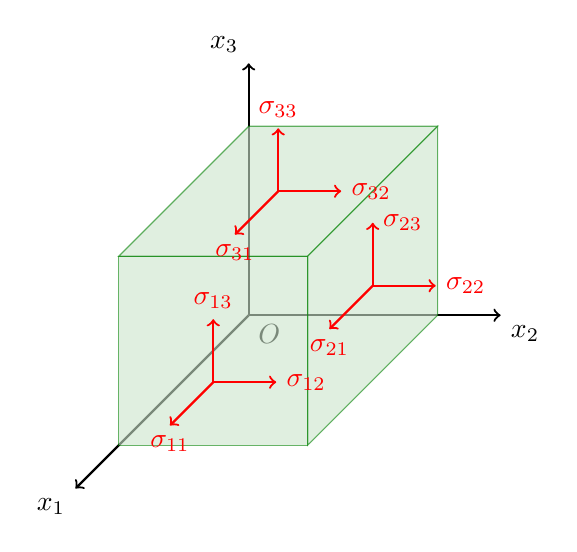
\begin{tikzpicture}[x={(-0.55cm, -0.55cm)}, y={(0.8cm, 0cm)}, z={(0cm, 0.8cm)}]
    \node[below right]{$O$}; 
    \draw[thick,->] (0,0,0) -- (4,0,0) node[anchor=north east]{$x_1$};
    \draw[thick,->] (0,0,0) -- (0,4,0) node[anchor=north west]{$x_2$};
    \draw[thick,->] (0,0,0) -- (0,0,4) node[anchor=south east]{$x_3$};
    \filldraw[draw=Green, fill=Green!20, opacity=0.6]
    (3,0,0) -- (3,3,0) -- (3,3,3) --  (3,0,3) -- cycle;
    \filldraw[draw=Green, fill=Green!20, opacity=0.6]
    (0,0,3) -- (0,3,3) -- (3,3,3) --  (3,0,3) -- cycle;
    \filldraw[draw=Green, fill=Green!20, opacity=0.6]
    (0,3,0) -- (3,3,0) -- (3,3,3) --  (0,3,3) -- cycle;
    \draw[red,thick,->] (3,1.5,1) -- (4,1.5,1) node[below]{$\sigma_{11}$};
    \draw[red,thick,->] (3,1.5,1) -- (3,2.5,1) node[right]{$\sigma_{12}$};
    \draw[red,thick,->] (3,1.5,1) -- (3,1.5,2) node[above]{$\sigma_{13}$};
    \draw[red,thick,->] (1.5,3,1.5) -- (2.5,3,1.5) node[below]{$\sigma_{21}$};
    \draw[red,thick,->] (1.5,3,1.5) -- (1.5,4,1.5) node[right]{$\sigma_{22}$};
    \draw[red,thick,->] (1.5,3,1.5) -- (1.5,3,2.5) node[right]{$\sigma_{23}$};
    \draw[red,thick,->] (1.5,1.5,3) -- (2.5,1.5,3) node[below]{$\sigma_{31}$};
    \draw[red,thick,->] (1.5,1.5,3) -- (1.5,2.5,3) node[right]{$\sigma_{32}$};
    \draw[red,thick,->] (1.5,1.5,3) -- (1.5,1.5,4) node[above]{$\sigma_{33}$};
    \end{tikzpicture} 
    \caption{The components of stress acting on a mass element.}
    \label{fig:stresscube}
\end{figure}
Since the traction, as a force, and the direction are both vectors, by the Quotient Law (Theorem \ref{thm:quotientl}), $\sigma_{ij}$ must be a rank-$2$ tensor. It is subsequently known as the \index{Cauchy Stress Tensor}\keywordhl{Cauchy Stress Tensor}. Now, we assume any mass element within a continuum (e.g. a rock layer) has to be in \textit{static equilibrium} so it is not moving. This specifically requires that there is no net torque that will rotate the mass element (presented as a parallelepiped in Figure \ref{fig:stresspiped}). The stresses on the opposite faces of the parallelepiped must then be equal in magnitude and opposite in direction. Take the $2,3$ directions as an illustration, the shear stresses on any pair of opposite faces (e.g.\ the component $\sigma_{23}$ on the $2$-planes) in another axis (e.g.\ in the $3$-direction) will generate a couple that tends to rotate the parallelepiped. To prevent the mass element from rotating, the shear stresses on the corresponding side faces (e.g.\ the component $\sigma_{32}$ on the $3$-planes) must balance this torque out, and thus $\sigma_{23} = \sigma_{32}$. By the same logic, $\sigma_{13} = \sigma_{31}$ and $\sigma_{12} = \sigma_{21}$, or more generally
\begin{align}
\sigma_{ij} = \sigma_{ji}
\end{align}
which means that the stress tensor is a symmetric one (this also means that the transpose in (\ref{eqn:cauchyT}) is not important). Moreover, as it is a tensor, it obeys the Transformation Law (Properties \ref{proper:translaw}) so that the change of coordinates will be
\begin{align}
\sigma'_{ij} = a_{ki}a_{lj}\sigma_{kl}
\end{align}
when viewed from the matrix perspective, it easily reminds us about orthogonal diagonalization (\ref{eqn:orthodiagonalPAP}) in Definition \ref{defn:orthodiagonal} since $a_{**}$ represents an orthogonal matrix and Theorem \ref{thm:symdiag} is applicable to the symmetric stress tensor. Therefore, we can always compute the orthonormal eigenvectors for any matrix representation of the stress tensor. After a change of coordinates via orthogonal diagonalization, these orthonormal eigenvectors will then become the \index{Principal Axes}\index{Principal Directions}\keywordhl{principal axes/directions} (akin to Theorem \ref{thm:PCA}) used in the new coordinate frame. The corresponding eigenvalues are naturally called the \index{Principal Stresses}\keywordhl{principal stresses} (denoted by $\sigma_{*}$ with one subscript only) and there will be no shearing components in the transformed representation of the stress tensor. Hence, the traction along any principal direction will be aligned with the normal to the surface and is equal to the respective principal stress. The geological convection is that compression/tension is taken to be positive/negative. For the ease of demonstration, we will consider plane stress with only $2$ directions first.

\begin{figure}
    \centering
    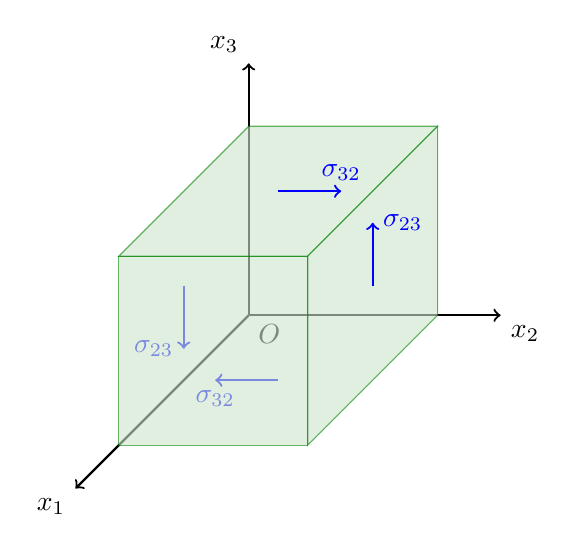
\begin{tikzpicture}[x={(-0.55cm, -0.55cm)}, y={(0.8cm, 0cm)}, z={(0cm, 0.8cm)}]
    \node[below right]{$O$}; 
    \draw[thick,->] (0,0,0) -- (4,0,0) node[anchor=north east]{$x_1$};
    \draw[thick,->] (0,0,0) -- (0,4,0) node[anchor=north west]{$x_2$};
    \draw[thick,->] (0,0,0) -- (0,0,4) node[anchor=south east]{$x_3$};
    \draw[blue,thick,->] (1.5,0,1.5) -- (1.5,0,0.5) node[left]{$\sigma_{23}$};
    \draw[blue,thick,->] (1.5,1.5,0) -- (1.5,0.5,0) node[below]{$\sigma_{32}$};
    \filldraw[draw=Green, fill=Green!20, opacity=0.6]
    (3,0,0) -- (3,3,0) -- (3,3,3) --  (3,0,3) -- cycle;
    \filldraw[draw=Green, fill=Green!20, opacity=0.6]
    (0,0,3) -- (0,3,3) -- (3,3,3) --  (3,0,3) -- cycle;
    \filldraw[draw=Green, fill=Green!20, opacity=0.6]
    (0,3,0) -- (3,3,0) -- (3,3,3) --  (0,3,3) -- cycle;
    \draw[blue,thick,->] (1.5,3,1.5) -- (1.5,3,2.5) node[right]{$\sigma_{23}$};
    \draw[blue,thick,->] (1.5,1.5,3) -- (1.5,2.5,3) node[above]{$\sigma_{32}$};
    \end{tikzpicture} 
    \caption{The balance between shear stresses along the $2,3$ ($yz$) cross-section for the mass element in Figure \ref{fig:stresscube}.}
    \label{fig:stresspiped}
\end{figure}

\begin{exmp}
For a two-dimensional stress tensor that has the components of (unit: \si{MPa})
\begin{align*}
\sigma =
\begin{bmatrix}
\sigma_{11} & \sigma_{12} \\
\sigma_{21} & \sigma_{22}
\end{bmatrix}
=
\begin{bmatrix}
5 & 1 \\
1 & 7
\end{bmatrix}
\end{align*}
find its principal stresses and principal directions.
\end{exmp}
\begin{solution}
We can directly compute the eigenvalues and eigenvectors, but we can do it in a more tricky way by recalling the results indicated by (\ref{eqn:rotate2dquadmat}) and (\ref{eqn:rotate2dquad}). The angle $\theta$ required to align the coordinate system is immediately inferred from 
\begin{align*}
\cot(2\theta) = \frac{5-7}{2} = -1
\end{align*}
which translates to $\theta = -\frac{\pi}{8}$, $\cos(\theta) = \frac{\sqrt{2+\sqrt{2}}}{2}$ and $\sin(\theta) = -\frac{\sqrt{2-\sqrt{2}}}{2}$. So the principal directions are at an angle of $\frac{\pi}{8}$ to the original axes. The principal stresses are then found by (\ref{eqn:rotate2dquadmat}) as well:
\begin{align*}
\begin{bmatrix}
\cos (-\frac{\pi}{8}) & \sin (-\frac{\pi}{8}) \\
-\sin (-\frac{\pi}{8}) & \cos (-\frac{\pi}{8})
\end{bmatrix}
\begin{bmatrix}
5 & 1 \\
1 & 7
\end{bmatrix}
\begin{bmatrix}
\cos (-\frac{\pi}{8}) & -\sin (-\frac{\pi}{8}) \\
\sin (-\frac{\pi}{8}) & \cos (-\frac{\pi}{8})
\end{bmatrix}
=    
\begin{bmatrix}
6-\sqrt{2} & 0 \\
0 & 6+\sqrt{2}
\end{bmatrix}
\end{align*}
So the principal stresses are $6-\sqrt{2} \approx \SI{4.59}{MPa}$ and $6+\sqrt{2} \approx \SI{7.41}{MPa}$. We will usually arrange the index from the largest to smallest stress so we will write them as $\sigma_1 = \SI{7.41}{MPa}$ and $\sigma_2 = \SI{4.59}{MPa}$ and this will require us to rotate the coordinate frame by an extra $\SI{90}{\degree}$.
\end{solution}
By reversing and extending the logic in (\ref{eqn:rotate2dquadmat}), a stress tensor that has been aligned in the principal directions and only has non-zero stress components along the main diagonal, can also undergo any rotation of degree $\theta$, resulting in
\begin{align}
\sigma'_{ij} &= 
\begin{bmatrix}
\cos \theta & \sin \theta \\
-\sin \theta & \cos \theta
\end{bmatrix}
\begin{bmatrix}
\sigma_1 & 0 \\
0 & \sigma_2 
\end{bmatrix}
\begin{bmatrix}
\cos \theta & -\sin \theta \\
\sin \theta & \cos \theta
\end{bmatrix} \nonumber \\
&=
\begin{bmatrix}
\cos \theta & \sin \theta \\
-\sin \theta & \cos \theta
\end{bmatrix}
\begin{bmatrix}
\sigma_1\cos \theta & -\sigma_1\sin \theta \\
\sigma_2\sin \theta & \sigma_2\cos \theta
\end{bmatrix} \nonumber \\
&=
\begin{bmatrix}
\sigma_1\cos^2 \theta + \sigma_2\sin^2\theta & -\sigma_1\sin \theta \cos\theta + \sigma_2\cos \theta\sin\theta \\
-\sigma_1\sin \theta\cos\theta + \sigma_2\sin\theta\cos\theta & \sigma_1\sin^2\theta + \sigma_2\cos^2 \theta
\end{bmatrix}
\end{align}
Rewriting the components using trigonometric identities simplifies them into
\begin{subequations}
\begin{align}
\sigma_{x'} = \sigma'_1 &= \sigma_1\cos^2 \theta + \sigma_2\sin^2\theta \nonumber \\
&= \sigma_1(\frac{1+\cos(2\theta)}{2}) + \sigma_2(\frac{1-\cos(2\theta)}{2}) \nonumber \\
&= \frac{\sigma_1 + \sigma_2}{2} + \frac{\sigma_1 - \sigma_2}{2}\cos(2\theta) \label{eqn:mohrnormal1} \\
\sigma_{y'} = \sigma'_2 &= \sigma_1\sin^2 \theta + \sigma_2\cos^2\theta \nonumber \\
&= \sigma_1(\frac{1-\cos(2\theta)}{2}) + \sigma_2(\frac{1+\cos(2\theta)}{2}) \nonumber \\
&= \frac{\sigma_1 + \sigma_2}{2} - \frac{\sigma_1 - \sigma_2}{2}\cos(2\theta) \label{eqn:mohrnormal2} \\
\tau_{x'y'} = \sigma'_{12} = \sigma'_{21} &= -\sigma_1\sin \theta \cos\theta + \sigma_2\cos \theta\sin\theta \nonumber \\
&= -\frac{\sigma_1 - \sigma_2}{2} \sin(2\theta) \label{eqn:mohrshear}
\end{align} 
\end{subequations}
where $\sigma_{x'}$ and $\sigma_{y'}$ are the normal tractions along the rotated axes and $\tau_{x'y'}$ is the shear traction. Notice that $\sigma_{x'}$ [or $\sigma_{y'}$] and $\tau_{x'y'}$ together form a circle parameterized by the double angle $2\theta$ with its center at $(\sigma, \tau) = (\frac{\sigma_1 + \sigma_2}{2}, 0)$ and a radius of $\frac{\sigma_1 - \sigma_2}{2}$.\footnote{$
(\sigma_{x'} - \frac{\sigma_1 + \sigma_2}{2})^2 + \tau_{x'y'}^2 = (\frac{\sigma_1 - \sigma_2}{2})^2\cos^2(2\theta) + (\frac{\sigma_1 - \sigma_2}{2})^2 \sin^2(2\theta) = (\frac{\sigma_1 - \sigma_2}{2})^2$}
Hence the information about normal/shear stresses on a surface of any orientation can be condensed into a circle centered at the horizontal axis that also cuts the horizontal axis at $\sigma = \sigma_1$ and $\sigma_2$ graphically. This is known as the \index{Mohr's Circle}\keywordhl{Mohr's Circle} and is illustrated in Figure \ref{fig:mohr1}. Bear in mind that when the geological convention is used, (\ref{eqn:mohrshear}) will have no negative sign, and an anti-clockwise [clockwise] rotation of the surface by a positive [negative] degree of $\theta$ will appear as an anti-clockwise [clockwise] rotation of the diameter within the Mohr's Circle by a positive [negative] degree $2\theta$ (double of the actual surface tilt). The largest shear traction will be obtained at a tilt of \SI{45}{\degree}.
 
\begin{figure}
\centering
    \begin{tikzpicture}
    \node[below left]{$O$}; 
    \coordinate (0) at (3,0);
    \draw[thick,->] (-2,0) -- (6,0) node[anchor=north east]{$\sigma_n$};
    \draw[thick,->] (0,-3) -- (0,3) node[anchor=north west]{$\tau$};
    \draw[Green, thick] (0) circle (2); 
    \filldraw[red] (1,0) circle (0.1) node[left]{$\sigma_2$}; 
    \filldraw[red] (5,0) circle (0.1) node(a)[right]{$\sigma_1$};
    \filldraw[blue] (0) ++ (40:2) circle (0.1); 
    \filldraw[blue] (0) ++ (220:2) circle (0.1);
    \draw[blue, thick] (0) -- ++(40:2) node(b)[above right]{$(\sigma_{x'}, \tau_{x'y'})$};
    \draw[blue, thick] (0) -- ++(220:2) node[below]{$(\sigma_{y'}, -\tau_{x'y'})$};
    \pic[->, draw, "$2\theta$", angle eccentricity=1.8] {angle = a--0--b};
    \end{tikzpicture}
    \caption{The schematic diagram of a Mohr's Circle.}
    \label{fig:mohr1}
\end{figure}

\begin{exmp}
For a two-dimensional plane with the principal stresses of $\sigma_1 = \SI{10}{MPa}$ and $\sigma_2 = \SI{5}{MPa}$, find the normal and shear tractions over the surface with a tilt of \SI{25}{\degree} from the principal axes in the positive direction.
\end{exmp}
\begin{solution}
The Mohr's Circle will have a radius of $\frac{\sigma_1 - \sigma_2}{2} = \frac{10-5}{2} = 2.5$, centered at $(\frac{\sigma_1 + \sigma_2}{2}, 0) = (\frac{10 + 5}{2}, 0) = (7.5,0)$ along the horizontal axis representing the normal direction. By (\ref{eqn:mohrnormal1}) and (\ref{eqn:mohrnormal2}) the normal tractions (in \si{MPa}) will be
\begin{align*}
\sigma_{x'}, \sigma_{y'} = 7.5 \pm 2.5 \cos(2(\SI{25}{\degree})) &= 7.5 \pm 2.5 \cos(\SI{50}{\degree}) \\
&= 7.5 \pm 1.61 = 9.11, 5.89
\end{align*}
and similarly the shear stress will be $\tau_{x'y'} = 2.5\sin(2(\SI{25}{\degree})) = \SI{1.92}{MPa}$ from (\ref{eqn:mohrshear}).
\end{solution}
Short Exercise: What are the new normal/shear tractions if the surface is further rotated by \SI{37}{\degree}?\footnote{This amounts to a net rotation of $(25+37)\si{\degree}= \SI{62}{\degree}$ so we simply repeat the calculation with $\theta = \SI{62}{\degree}$. The results should be $\sigma_{x'}, \sigma_{y'} = 7.5 \pm 2.5 \cos(2(\SI{62}{\degree})) = 7.5 \pm 2.5 \cos(\SI{124}{\degree}) = 7.5 \mp 1.40 = 6.10, 8.90$ and $\tau_{x'y'} = 2.5\sin(\SI{124}{\degree}) = 2.07$. Graphically, we can just rotate the previous diameter by an extra of $2 \times \SI{37}{\degree} = \SI{74}{\degree}$ on the Mohr's Circle.}

The generalization of Mohr's Circle to a three-dimensional volume can be done by first assuming that the coordinate system has been properly rotated to coincide with the three principal directions. Denote the respective principal stresses by $\sigma_1, \sigma_2, \sigma_3$ where they are arranged in descending order $\sigma_1 \geq \sigma_2 \geq \sigma_3$. Then given a normal $\hat{n} = n_i$ to the plane, the net traction is given by Cauchy's Formula (\ref{eqn:cauchyT}):
\begin{align}
\begin{bmatrix}
T_1 \\
T_2 \\
T_3
\end{bmatrix}  
=
\begin{bmatrix}
\sigma_{1} & 0 & 0 \\
0 & \sigma_{2} & 0 \\
0 & 0 & \sigma_{3}
\end{bmatrix}
\begin{bmatrix}
n_1 \\
n_2 \\
n_3
\end{bmatrix}
=
\begin{bmatrix}
\sigma_1 n_1 \\
\sigma_2 n_2 \\
\sigma_3 n_3
\end{bmatrix}    
\end{align}
and considering the squared magnitude of the traction, which is simply the sum of the squared magnitudes of the normal traction $\sigma_n$ and shear traction $\tau$, we have
\begin{align}
\sigma_n^2 + \tau^2 = \norm{T}^2 = T_1^2 + T_2^2 + T_3^2 = \sigma_1^2 n_1^2 + \sigma_2^2 n_2^2 + \sigma_3^2 n_3^2 \label{eqn:mohr3d1}
\end{align}
where the normal traction is simply
\begin{align}
\sigma_n = (\sigma_1 n_1, \sigma_2 n_2, \sigma_3 n_3)^T \cdot (n_1, n_2, n_3)^T = \sigma_1n_1^2 + \sigma_2n_2^2 + \sigma_3n_3^2 \label{eqn:mohr3d2}
\end{align}
Finally, we have a quite trivial condition of $\hat{n}$ being a unit normal vector:
\begin{align}
1 = n_1^2 + n_2^2 + n_3^2 \label{eqn:mohr3d3}
\end{align}
(\ref{eqn:mohr3d1}), (\ref{eqn:mohr3d2}), (\ref{eqn:mohr3d3}) together form a linear system of three equations in three unknowns $n_1^2, n_2^2, n_3^2$. This can be efficiently dealt with with Cramer's Rule. Considering the first unknown $n_1^2$, we have
\begin{align}
n_1^2 &= \frac{\begin{vmatrix}
\sigma_n^2 + \tau^2 & \sigma_2^2 & \sigma_3^2 \\
\sigma_n & \sigma_2 & \sigma_3 \\
1 & 1 & 1
\end{vmatrix}}
{\begin{vmatrix}
\sigma_1^2 & \sigma_2^2 & \sigma_3^2 \\
\sigma_1 & \sigma_2 & \sigma_3 \\
1 & 1 & 1    
\end{vmatrix}} \nonumber \\
&= \frac{[(\sigma_n^2 + \tau^2)\sigma_2 + \sigma_2^2 \sigma_3 + \sigma_n\sigma_3^2] - [\sigma_2\sigma_3^2 + \sigma_3(\sigma_n^2 + \tau^2) + \sigma_n\sigma_2^2]}{(\sigma_1^2\sigma_2 + \sigma_2^2\sigma_3 + \sigma_3^2\sigma_1) - (\sigma_2\sigma_3^2 + \sigma_3\sigma_1^2 + \sigma_1\sigma_2^2)} \nonumber \\
&= \frac{(\sigma_n^2 + \tau^2)(\sigma_2 - \sigma_3) - \sigma_n(\sigma_2^2 - \sigma_3^2)+(\sigma_2^2\sigma_3 - \sigma_2\sigma_3^2)}{(\sigma_1^2\sigma_2 + \sigma_2^2\sigma_3 + \sigma_3^2\sigma_1 + \sigma_1\sigma_2\sigma_3) - (\sigma_2\sigma_3^2 + \sigma_3\sigma_1^2 + \sigma_1\sigma_2^2 + \sigma_1\sigma_2\sigma_3)} \nonumber \\
&= \frac{(\sigma_n^2 + \tau^2)(\sigma_2 - \sigma_3) - \sigma_n(\sigma_2 + \sigma_3)(\sigma_2 - \sigma_3) + \sigma_2\sigma_3(\sigma_2 - \sigma_3)}{(\sigma_1 - \sigma_2)(\sigma_2 - \sigma_3)(\sigma_1-\sigma_3)} \nonumber \\
&= \frac{(\sigma_n^2 + \tau^2) - \sigma_n(\sigma_2 + \sigma_3) + \sigma_2\sigma_3}{(\sigma_1 - \sigma_2)(\sigma_1-\sigma_3)}
\end{align}
Since $n_1^2 \geq 0$, $\sigma_1 - \sigma_2 \geq 0$ and $\sigma_1 - \sigma_3 \geq 0$, we have
\begin{align}
(\sigma_n^2 + \tau^2) - \sigma_n(\sigma_2 + \sigma_3) + \sigma_2\sigma_3 &\geq 0 \nonumber \\
(\sigma_n-\frac{\sigma_2 + \sigma_3}{2})^2 + \tau^2 + \sigma_2\sigma_3 - (\frac{\sigma_2 + \sigma_3}{2})^2 &\geq 0 \nonumber \\
(\sigma_n-\frac{\sigma_2 + \sigma_3}{2})^2 + \tau^2 &\geq (\frac{\sigma_2 + \sigma_3}{2})^2 - \sigma_2\sigma_3 \nonumber \\
&= \frac{\sigma_2^2}{4} + \frac{\sigma_2\sigma_3}{2} +\frac{\sigma_3^2}{4} - \sigma_2\sigma_3 \nonumber \\
&= \frac{\sigma_2^2}{4} - \frac{\sigma_2\sigma_3}{2} +\frac{\sigma_3^2}{4} \nonumber \\
&= (\frac{\sigma_2 - \sigma_3}{2})^2
\end{align}
by completing squares. Therefore, the normal and shear traction must lie outside the Mohr's Circle centered at $(\frac{\sigma_2 + \sigma_3}{2},0)$ with a radius of $\frac{\sigma_2 - \sigma_3}{2}$, which represents a circle that lies along the horizontal (normal traction) axis and cuts it at $\sigma_n = \sigma_2$ and $\sigma_3$. Similarly, we leave it to the readers to check that
\begin{align}
n_2^2 &= \mathcolor{red}{-}\frac{(\sigma_n^2 + \tau^2) - \sigma_n(\sigma_1 + \sigma_3) + \sigma_1\sigma_3}{(\sigma_1 - \sigma_2)(\sigma_2-\sigma_3)} \\
n_3^2 &= \frac{(\sigma_n^2 + \tau^2) - \sigma_n(\sigma_1 + \sigma_2) + \sigma_1\sigma_2}{(\sigma_2 - \sigma_3)(\sigma_1-\sigma_3)}
\end{align}
(notice the negative sign for $n_2^2$, why?) and thus along the same lines, we have
\begin{align}
(\sigma_n-\frac{\sigma_1 + \sigma_3}{2})^2 + \tau^2 &\mathcolor{red}{\leq} (\frac{\sigma_1 - \sigma_3}{2})^2 \\
(\sigma_n-\frac{\sigma_1 + \sigma_2}{2})^2 + \tau^2 &\geq (\frac{\sigma_1 - \sigma_2}{2})^2
\end{align}
So the normal and shear traction must also fall outside the Mohr's Circle centered at $(\frac{\sigma_1 + \sigma_2}{2},0)$ with a radius of $\frac{\sigma_1 - \sigma_2}{2}$ that cuts the horizontal axis at $\sigma_n = \sigma_1$ and $\sigma_2$, but inside the larger Mohr's Circle also centered at the horizontal axis that cuts it at $\sigma_n = \sigma_1$ and $\sigma_3$. These are demonstrated in Figure \ref{fig:mohr3d}.

\begin{figure}
    \centering
    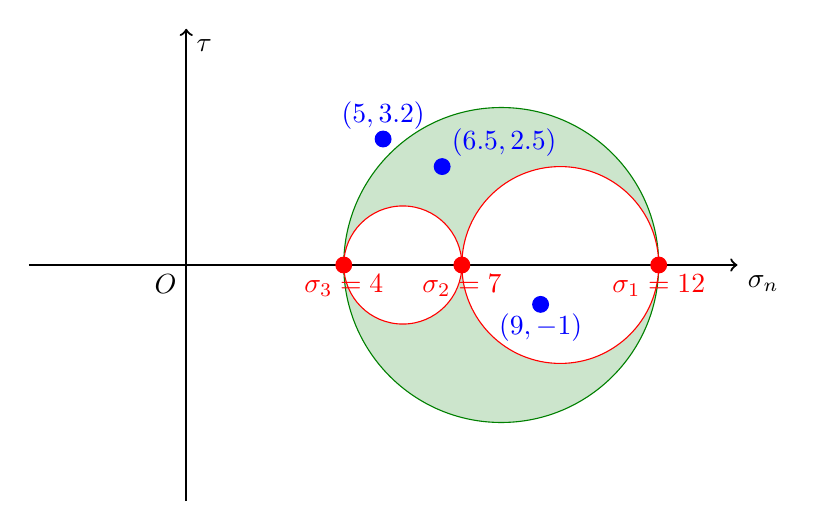
\begin{tikzpicture}
    \node[below left]{$O$}; 
    \draw[Green,fill=Green!20] (4,0) circle (2);
    \draw[red,fill=white] (2.75,0) circle (0.75);
    \draw[red,fill=white] (4.75,0) circle (1.25);
    \draw[thick,->] (-2,0) -- (7,0) node[anchor=north west]{$\sigma_n$};
    \draw[thick,->] (0,-3) -- (0,3) node[anchor=north west]{$\tau$};
    \filldraw[red] (2,0) circle (0.1) node[below]{$\sigma_3 = 4$};
    \filldraw[red] (3.5,0) circle (0.1) node[below]{$\sigma_2 = 7$};
    \filldraw[red] (6,0) circle (0.1) node[below]{$\sigma_1 = 12$};
    \filldraw[blue] (4.5,-0.5) circle (0.1) node[below]{$(9,-1)$};
    \filldraw[blue] (3.25,1.25) circle (0.1) node[above right]{$(6.5,2.5)$};
    \filldraw[blue] (2.5,1.6) circle (0.1) node[above]{$(5,3.2)$};
    \end{tikzpicture}
    \caption{Mohr's Circles extended to the three-dimensional space, adapted to Example \ref{exmp:mohr3d}. The normal/shear tractions $(\sigma_n, \tau)$ have to lie within the shaded region.}
    \label{fig:mohr3d}
\end{figure}

\begin{exmp}
\label{exmp:mohr3d}
For a three-dimensional volume with principal stresses of $\sigma_1 = 12$, $\sigma_2 = 7$, $\sigma_3 = 4$ (in MPa), check if the following pairs of normal/shear tractions $(\sigma_n, \tau)$ are valid.
\begin{enumerate}[label=(\alph*)]
    \item $(9,-1)$
    \item $(6.5,2.5)$
    \item $(5,3.2)$
\end{enumerate}
\end{exmp}
\begin{solution}
Figure \ref{fig:mohr3d} has been drawn for the situation in this question. We simply mark the locations for the traction pairs and see if the dots fall within the shaded region bounded by the three Mohr's Circles. The direct visual inspection shows that the second pair is possible but the first and last pairs are not valid.
\end{solution}
We note that the largest shear traction is acquired when the surface is inclined at $\SI{45}{\degree}$ just between the first and third principal planes, similar to the plane stress scenario.

\subsection{Eulerian and Lagrangian Views, Spatial and Material Derivatives}

In Continuum Mechanics, the continuum may deform and move along the flow. Due to this, we have two descriptions of the continuum: \textit{Eulerian} and \textit{Lagrangian} descriptions. Given a property $P$ of the continuum, in the \index{Eulerian Description}\index{Spatial Description}\keywordhl{Eulerian (spatial) description}, we retrieve the value of $P$ by referring to the local coordinates $\textbf{x} = x_i$ at the current time $t$, so that $P = P(x_i, t)$. This is more commonly used in many situations because of convenience. However, sometimes we also need the \index{Lagrangian Description}\index{Material Description}\keywordhl{Lagrangian (material) description} that essentially follows a mass particle. We need to "label" the particle with reference coordinates $\textbf{X} = X_i$ (in capital letters) which are the local coordinates recorded at some reference time $t_0$, such that $X_i = x_i(t_0)$. In this case, the value of $P$ is evaluated by going back to the fixed reference coordinates, and hence we have $P = P(X_i, t)$ instead. It is possible to convert between these two descriptions by
\begin{subequations}
\begin{align}
x_i = x_i(X_i, t) \label{eqn:lagtoeuler}
\end{align}
which extracts the current local coordinates using labels from the Lagrangian description, and vice versa
\begin{align}
X_i = X_i(x_i, t)    
\end{align}
\end{subequations}
which returns the labeled coordinates using the Eulerian description. This leads to the \index{Displacement Field}\keywordhl{displacement field}
\begin{align}
u_i = x_i - X_i
\end{align}
which is the displacement between the current position of particles and their initial reference position. The \index{Material Displacement Gradient}\keywordhl{material displacement gradient} is the displacement differentiated with respect to the material coordinates:
\begin{align}
\frac{\partial u_i}{\partial X_j} = \frac{\partial x_i}{\partial X_j} -  \frac{\partial X_i}{\partial X_j} = \frac{\partial x_i}{\partial X_j} - \delta_{ij}
\end{align}
Similarly, we also have the \index{Spatial Displacement Gradient}\keywordhl{spatial displacement gradient} that comes from differentiating the displacement with respect to the spatial coordinates:
\begin{align}
\frac{\partial u_i}{\partial x_j} = \frac{\partial x_i}{\partial x_j} -  \frac{\partial X_i}{\partial x_j} = \delta_{ij} - \frac{\partial X_i}{\partial x_j}
\end{align}
Both of them are rank-$2$ tensors.\footnote{We only show that for the first one but the second one is very similar. Note that by the multivariable Chain Rule
\begin{align*}
(\frac{\partial u_i}{\partial X_j})dX_j = du_i
\end{align*}
Since $dX_j$ and $du_i$ are (differentials of) displacement and velocity, they are vectors and an immediate use of the Quotient Law (Theorem \ref{thm:quotientl}) shows that $\partial u_i/\partial X_j$ has to be a rank-$2$ tensor.} A comparison of these two descriptions is given in Figure \ref{fig:displace}.
\begin{figure}
    \centering
    \begin{tikzpicture}
    \node[below left]{$O$}; 
    \draw[thick,->] (0,0) -- (9,0);
    \draw[thick,->] (0,0) -- (0,5);
    \draw[dashed] (1,1) to [in=210, out=70] (1,3) to [in=100, out=30] (2,3) to [in=45, out=-80] (2,1) to [in=250, out=225] cycle;
    \node at (1,3.5) {Reference};
    \draw[thick] (4.5,2) to [out=100, in=-100] (4,4.5) to [out=80, in=160] (6.5,5) to [out=-20, in=45] (6,1.5) to [out=-135, in=-80] cycle;
    \node at (6,1) {Current};
    \draw[blue, -{Latex[length=3mm]}] (0,0) -- (1.4, 1.6) node[midway, sloped, below]{$\textbf{X}$};
    \draw[blue, -{Latex[length=3mm]}] (0,0) -- (1.3, 2.5) node[pos=0.7, sloped, above]{$\textbf{X} + d\textbf{X}$};
    \draw[red, -{Latex[length=3mm]}] (1.4, 1.6) -- (5.1, 2.6) node[pos=0.7, sloped, above]{$\textbf{u}$};
    \draw[red, -{Latex[length=3mm]}] (1.3, 2.5) -- (5.9, 4.3) node[pos=0.4, sloped, above]{$\textbf{u} + d\textbf{u}$};
    \draw[Green, -{Latex[length=3mm]}] (5.1, 2.6) -- (5.9, 4.3) node[midway, right]{$d\textbf{x}$};
    \draw[Green, -{Latex[length=3mm]}] (0,0) -- (5.1, 2.6) node[pos=0.65, sloped, below]{$\textbf{x}$};
    \draw[Green, -{Latex[length=3mm]}] (0,0) -- (5.9, 4.3) node[midway, sloped, above]{$\textbf{x} + d\textbf{x}$};
    \draw[blue, -{Latex[length=3mm]}] (1.4, 1.6) -- (1.3, 2.5) node[midway, right]{$d\textbf{X}$};
    \filldraw[black] (1.4, 1.6) circle (0.1) node[blue, below, xshift=4pt]{$A_0$};
    \filldraw[black] (1.3, 2.5) circle (0.1) node[blue, above]{$B_0$};
    \filldraw[black] (5.1, 2.6) circle (0.1) node[Green, below]{$A$};
    \filldraw[black] (5.9, 4.3) circle (0.1) node[Green, above]{$B$};
    \end{tikzpicture}
    \caption{The conversion between the Eulerian/Lagrangian views for coordinates and displacements.}
    \label{fig:displace}
\end{figure}
Notice that the quantity $\partial x_i/\partial X_j$ (also the closely related $\partial X_i/\partial x_j$) appeared in the displacement gradient. This is called the \index{Deformation Jacobian}\keywordhl{Jacobian} of the deformation. To see this, by the multivariable Chain Rule, the transformation between the Eulerian and Lagrangian displacements is explicitly
\begin{subequations}
\begin{empheq}[left={\empheqlbrace}]{alignat=1}
d\textbf{x}_1 &= \frac{\partial x_1}{\partial X_1}dX_1\textbf{e}_1 + \frac{\partial x_1}{\partial X_2}dX_2\textbf{e}_2 + \frac{\partial x_1}{\partial X_3}dX_3\textbf{e}_3 \\
d\textbf{x}_2 &= \frac{\partial x_2}{\partial X_1}dX_1\textbf{e}_1 + \frac{\partial x_2}{\partial X_2}dX_2\textbf{e}_2 + \frac{\partial x_2}{\partial X_3}dX_3\textbf{e}_3 \\
d\textbf{x}_3 &= \frac{\partial x_3}{\partial X_1}dX_1\textbf{e}_1 + \frac{\partial x_3}{\partial X_2}dX_2\textbf{e}_2 + \frac{\partial x_3}{\partial X_3}dX_3\textbf{e}_3 
\end{empheq}
\end{subequations}
The deformed Eulerian volume $dV$ for an infinitesimally small mass is then given by (\ref{eqn:scalartriple}) from Properties \ref{proper:parallelpiped}.
\begin{align}
(d\textbf{x}_1 \times d\textbf{x}_2) \cdot d\textbf{x}_3 &= 
\begin{vmatrix}
\dfrac{\partial x_1}{\partial X_1}dX_1 & \dfrac{\partial x_1}{\partial X_2}dX_2 & \dfrac{\partial x_1}{\partial X_3}dX_3 \\[10pt] 
\dfrac{\partial x_2}{\partial X_1}dX_1 & \dfrac{\partial x_2}{\partial X_2}dX_2 & \dfrac{\partial x_2}{\partial X_3}dX_3 \\[10pt] 
\dfrac{\partial x_3}{\partial X_1}dX_1 & \dfrac{\partial x_3}{\partial X_2}dX_2 & \dfrac{\partial x_3}{\partial X_3}dX_3 \\[10pt] 
\end{vmatrix} \nonumber \\
&= \det(\frac{\partial x_i}{\partial X_j}) dX_1dX_2dX_3 = JdV_0
\end{align}
where $dV_0 = dX_1dX_2dX_3$ is the infinitesimal reference Lagrangian volume differential and 
\begin{align}
J = \det(\frac{\partial x_i}{\partial X_j}) \label{eqn:Jacdet} 
\end{align} is the determinant of the Jacobian. Alternatively, using the Index Notation and epsilon symbol, we can also arrive at
\begin{align}
dV &= \epsilon_{lmn} dx_ldx_mdx_n \nonumber \\
&= \epsilon_{lmn} \frac{\partial x_l}{\partial X_i}\frac{\partial x_m}{\partial X_j}\frac{\partial x_n}{\partial X_k} dX_idX_jdX_k & \text{(Multivariable Chain Rule)} \nonumber \\
&= \epsilon_{ijk} J dX_idX_jdX_k & \text{(by (\ref{eqn:determinanteps2}) and (\ref{eqn:Jacdet}))} \nonumber \\
&= J dV_0 \label{eqn:dVJdV_0}
\end{align}
Consequentially, $J$ is the ratio of the reference to the current volume. Due to the conservation of matter, the deformed volume cannot vanish if the initial reference volume is finite and vice versa. This implies that the determinant of the Jacobian (or simply called Jacobian from now on) cannot vanish, i.e.\ $J = \det(\partial x_i/\partial X_j) \neq 0$. This ensures that the conversion between the Eulerian and Lagrangian descriptions is one-to-one.\par

Now, we are going to examine the time derivative of a tensor quantity $P = P_{ij\ldots}$ from both the Eulerian and Lagrangian views. Using the Lagrangian description, it can be expressed as $P = P(\textbf{X}, t)$ where $\textbf{X}$ represents the reference coordinates. The \index{Material Derivative}\keywordhl{material derivative} $dP/dt$ is the rate of change in $P$ following a particle with respect to time $t$. Since the reference coordinates of the tracked particle are essentially labels that do not change with time, the material derivative of $P(\textbf{X}, t)$ in the Lagrangian framework is simply
\begin{align}
\frac{d}{dt} P(\textbf{X},t) = \frac{\partial}{\partial t} P(\textbf{X},t) \label{eqn:lagpartialt}
\end{align}
its partial derivative with respect to time. However, in the Eulerian description, we use the current coordinates of the particle that will change in time such that $P = P(\textbf{x}, t)$ and $\textbf{x} = \textbf{x}(\textbf{X}, t)$, and thus the material derivative has to be obtained using the multivariable Chain Rule as
\begin{align}
\underbrace{\frac{d}{dt} P(\textbf{x},t)}_{\text{Material}} &= \frac{\partial}{\partial t} P(\textbf{x},t) + \frac{\partial}{\partial x_k} [P(\textbf{x},t)] \frac{dx_k}{dt} \nonumber \\
&= \underbrace{\frac{\partial}{\partial t} P(\textbf{x},t)}_{\text{Spatial}} + \underbrace{v_k\frac{\partial}{\partial x_k} [P(\textbf{x},t)]}_{\text{Advective}} 
\end{align}
where $d\textbf{x}/dt = dx_k/dt = v_k = \textbf{v}$ are the velocities of the particle. This shows that the material derivative is the combined effects of the \index{Spatial Derivative}\keywordhl{spatial derivative} which is the local rate of change of $P$ fixed at the present position of the particle, and the \index{Advective Derivative}\keywordhl{advective derivative} which is the rate of change of $P$ attributed to the particle being advected along the gradient of the field of $P$ due to the flow. Accordingly, the material derivative operator expressed in the Eulerian spatial description is given by 
\begin{align}
\frac{d}{dt} = \frac{\partial}{\partial t} + v_k\frac{\partial}{\partial x_k} = \frac{\partial}{\partial t} + \textbf{v} \cdot \nabla \label{eqn:localmatderiv}
\end{align}
Going in the reverse direction, it implies that the evolution of some property measured at a fixed point in space (spatial) is the actual change imparted to the particle (material) subtracted by the apparent advective effect due to its motion. The relationship between these three terms is demonstrated in Figure \ref{fig:advection} in a one-dimensional setting.
\begin{figure}[ht!]
    \centering
    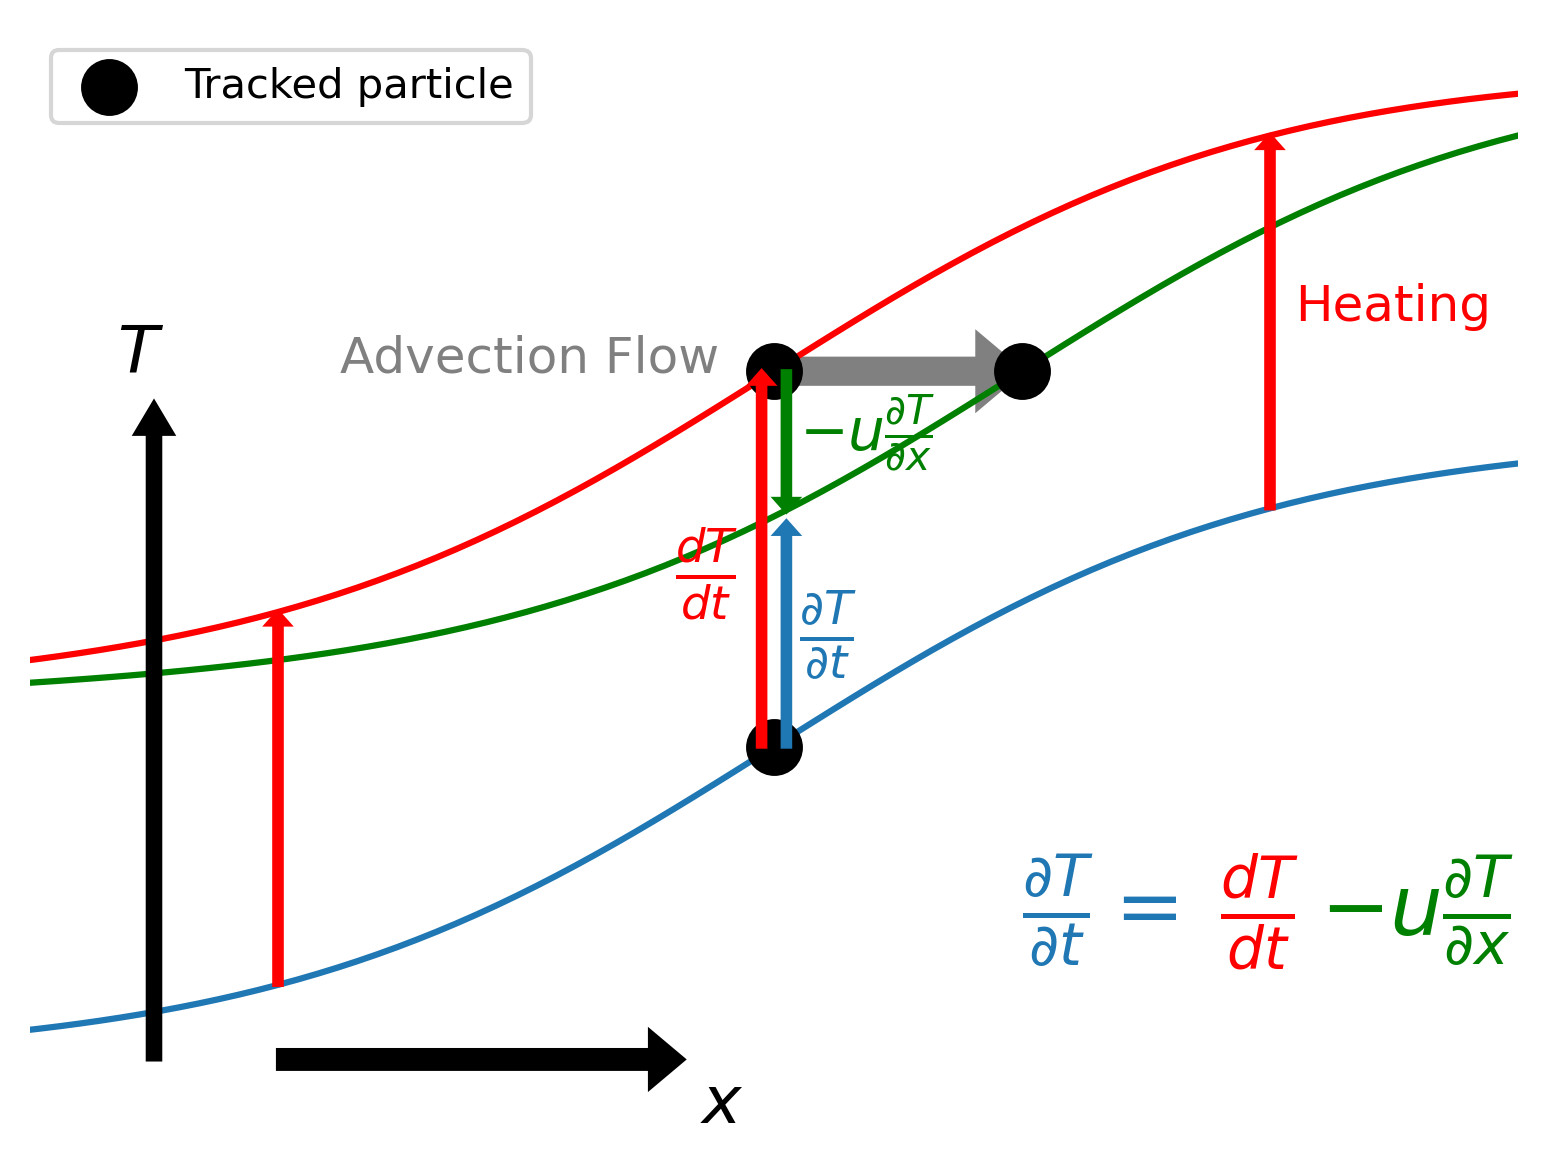
\includegraphics[scale=0.8]{graphics/advect.png}
    \caption{The relationship between the spatial (blue) and material derivative (red) alongside the advective term (green), where we use temperature $T$ as the variable and only look at a single direction $x$ (and velocity $u$) for demonstration.}
    \label{fig:advection}
\end{figure}

\subsection{Field Equations}
In this subsection, we will proceed to derive several \index{Field Equations}\keywordhl{field equations} which govern the dynamics of physical fields like temperature and motion. The central ingredient for the derivation is the \textit{conservation of mass}, and we will consider the mass contained in a volume bounded by an arbitrary closed surface. The boundary of this volume will be assumed to move alongside the particles on it and thus it is a \index{Material Volume}\keywordhl{material volume}. Therefore, it will contain the same set of particles for all time. Considering this material volume, the amount of mass inside it can be expressed as an integral over the deformed volume in the current configuration as
\begin{align}
m = \int_{V(t)} \rho(\textbf{x},t) dV \label{eqn:eulermass}
\end{align}
where $V(t)$ represents the current volume and $\rho(\textbf{x},t)$ is the density field in the Eulerian frame, both of which can change with time. However, we can also switch to the Lagrangian frame where the mass integral is taken over a fixed reference volume $V_0 = V(t_0)$, which coincides with the material volume of the mass at some reference time. Moreover, at the reference time, the density will no longer depend on time and will only vary in the reference coordinates, i.e.\ $\rho_0 = \rho_0(\textbf{X}) = \rho(\textbf{x}(\textbf{X},t_0), t_0)$. Therefore, an alternative form of the mass integral will be
\begin{align}
m = \int_{V_0} \rho_0(\textbf{X}) dV_0 \label{eqn:lagmass}
\end{align}
The principle of \index{Conservation of Mass}\keywordhl{conservation of mass} requires that mass can neither be created nor destroyed and thus the mass within a material volume will remain the same at any time. As a result, the rate of change in mass must vanish, i.e. $dm/dt = 0$. Using this on (\ref{eqn:eulermass}) then leads to
\begin{align}
\frac{d}{dt}(\int_{V(t)} \rho(\textbf{x},t) dV) = 0
\end{align}
The problem with this formulation is that the integration volume, in addition to the density, depends on the time and the computation will be difficult. However, we can carry out a coordinate transformation from the Eulerian to the Lagrangian frame by (\ref{eqn:dVJdV_0}) to convert the integral from a moving volume to a reference volume as
\begin{align}
\frac{d}{dt}\left(\int_{V_0} \rho(\textbf{x}(\textbf{X},t),t) JdV_0 \right) = 0 \label{eqn:eulermassdt}   
\end{align}
Compared to (\ref{eqn:lagmass}), the density can now change with time as the condition is relaxed using (\ref{eqn:lagtoeuler}) to compute the current density using the reference coordinates. To proceed, we would like to do the time derivative under the integral sign and this requires us to know how to evaluate $dJ/dt$ first, which is the time derivative of the Jacobian. The Jacobian as a determinant, can be expressed in the Index Notation
\begin{align}
J = \epsilon_{ijk} \frac{\partial x_1}{\partial X_i}\frac{\partial x_2}{\partial X_j}\frac{\partial x_3}{\partial X_k} \label{eqn:Jdefn}
\end{align}
via (\ref{eqn:determinanteps3}) where $\partial x_l/\partial X_i$ is the Jacobian in the matrix/tensor form. Since the partial derivatives in the Jacobian are defined with respect to the material reference coordinates, the time derivative of the Jacobian can be done directly. Using the Product Rule, we have
\begin{align}
\frac{dJ}{dt} =  \epsilon_{ijk} [\frac{d}{dt}(\frac{\partial x_1}{\partial X_i})\frac{\partial x_2}{\partial X_j}\frac{\partial x_3}{\partial X_k} +  \frac{\partial x_1}{\partial X_i}\frac{d}{dt}(\frac{\partial x_2}{\partial X_j})\frac{\partial x_3}{\partial X_k} +  \frac{\partial x_1}{\partial X_i}\frac{\partial x_2}{\partial X_j}\frac{d}{dt}(\frac{\partial x_3}{\partial X_k})]
\label{eqn:dJdt1}
\end{align}
Note that in the material coordinates, by (\ref{eqn:lagpartialt}) the time derivative can be treated as a partial derivative, and by \index{Clairaut's Theorem}\keywordhl{Clairaut's Theorem} in Multivariable Calculus we can exchange the order of partial derivatives if they are smooth enough. Therefore, we have
\begin{align}
\frac{d}{dt}\frac{\partial x_l}{\partial X_i} = \frac{\partial}{\partial t}\frac{\partial x_l}{\partial X_i} = \frac{\partial}{\partial X_i}\frac{\partial x_l}{\partial t} = \frac{\partial}{\partial X_i}(\frac{d x_l}{dt}) = \frac{\partial v_l}{\partial X_i}
\end{align}
Now, we invoke the Eulerian description and introduce the current coordinates, such that
\begin{align}
\frac{\partial v_l}{\partial X_i} = \frac{\partial v_l}{\partial x_p}\frac{\partial x_p}{\partial X_i}
\end{align}
Take the first term in (\ref{eqn:dJdt1}) to illustrate, it becomes
\begin{align}
\epsilon_{ijk} \frac{d}{dt}(\frac{\partial x_1}{\partial X_i})\frac{\partial x_2}{\partial X_j}\frac{\partial x_3}{\partial X_k} = \epsilon_{ijk} \frac{\partial v_1}{\partial X_i}\frac{\partial x_2}{\partial X_j}\frac{\partial x_3}{\partial X_k} = \epsilon_{ijk} \frac{\partial v_1}{\partial x_p}\frac{\partial x_p}{\partial X_i}\frac{\partial x_2}{\partial X_j}\frac{\partial x_3}{\partial X_k} 
\end{align}
Notice that
\begin{align*}
\epsilon_{ijk} \frac{\partial x_p}{\partial X_i}\frac{\partial x_2}{\partial X_j}\frac{\partial x_3}{\partial X_k}
\end{align*}
will only give the non-zero Jacobian determinant if $p=1$, since when $p=2,3$ the rows of the determinant will be identical and hence
\begin{align}
\epsilon_{ijk} \frac{\partial v_1}{\partial x_p}\frac{\partial x_p}{\partial X_i}\frac{\partial x_2}{\partial X_j}\frac{\partial x_3}{\partial X_k} =  \frac{\partial v_1}{\partial x_1}(\epsilon_{ijk}\frac{\partial x_1}{\partial X_i}\frac{\partial x_2}{\partial X_j}\frac{\partial x_3}{\partial X_k}) = \frac{\partial v_1}{\partial x_1}J
\end{align}
where we have used the definition of $J$ in (\ref{eqn:Jdefn}). We can also show this by writing out the determinants in full as in (\ref{eqn:determinanteps3}):
\begin{align*}
&\quad\epsilon_{ijk} (\frac{\partial v_1}{\partial x_p}\frac{\partial x_p}{\partial X_i})\frac{\partial x_2}{\partial X_j}\frac{\partial x_3}{\partial X_k} \\
&= \small\begin{vmatrix}
\dfrac{\partial v_1}{\partial x_p}\dfrac{\partial x_p}{\partial X_1} & \dfrac{\partial v_1}{\partial x_p}\dfrac{\partial x_p}{\partial X_2} & \dfrac{\partial v_1}{\partial x_p}\dfrac{\partial x_p}{\partial X_3} \\[10pt]
\dfrac{\partial x_2}{\partial X_1} & \dfrac{\partial x_2}{\partial X_2} & \dfrac{\partial x_2}{\partial X_3} \\[10pt]
\dfrac{\partial x_3}{\partial X_1} & \dfrac{\partial x_3}{\partial X_2} & \dfrac{\partial x_3}{\partial X_3} 
\end{vmatrix} \\
&= \frac{\partial v_1}{\partial x_1}\small\begin{vmatrix}
\dfrac{\partial x_1}{\partial X_1} & \dfrac{\partial x_1}{\partial X_2} & \dfrac{\partial x_1}{\partial X_3} \\[10pt]
\dfrac{\partial x_2}{\partial X_1} & \dfrac{\partial x_2}{\partial X_2} & \dfrac{\partial x_2}{\partial X_3} \\[10pt]
\dfrac{\partial x_3}{\partial X_1} & \dfrac{\partial x_3}{\partial X_2} & \dfrac{\partial x_3}{\partial X_3} 
\end{vmatrix} +
\frac{\partial v_1}{\partial x_2}\small\begin{vmatrix}
\dfrac{\partial x_2}{\partial X_1} & \dfrac{\partial x_2}{\partial X_2} & \dfrac{\partial x_2}{\partial X_3} \\[10pt]
\dfrac{\partial x_2}{\partial X_1} & \dfrac{\partial x_2}{\partial X_2} & \dfrac{\partial x_2}{\partial X_3} \\[10pt]
\dfrac{\partial x_3}{\partial X_1} & \dfrac{\partial x_3}{\partial X_2} & \dfrac{\partial x_3}{\partial X_3} 
\end{vmatrix} +
\frac{\partial v_1}{\partial x_3}\small\begin{vmatrix}
\dfrac{\partial x_3}{\partial X_1} & \dfrac{\partial x_3}{\partial X_2} & \dfrac{\partial x_3}{\partial X_3} \\[10pt]
\dfrac{\partial x_2}{\partial X_1} & \dfrac{\partial x_2}{\partial X_2} & \dfrac{\partial x_2}{\partial X_3} \\[10pt]
\dfrac{\partial x_3}{\partial X_1} & \dfrac{\partial x_3}{\partial X_2} & \dfrac{\partial x_3}{\partial X_3} 
\end{vmatrix} \\
&= \frac{\partial v_1}{\partial x_1} J + \frac{\partial v_1}{\partial x_2}(0) + \frac{\partial v_1}{\partial x_3} (0) = \frac{\partial v_1}{\partial x_1} J \\
&\quad \text{(Properties \ref{proper:zerodet})}
\end{align*}
By the same reasoning, the second and third terms in (\ref{eqn:dJdt1}) will equal to
$(\partial v_2/\partial x_2)J$ and $(\partial v_3/\partial x_3)J$. So finally (\ref{eqn:dJdt1}) is reduced to simply
\begin{align}
\frac{dJ}{dt} = (\frac{\partial v_1}{\partial x_1} + \frac{\partial v_2}{\partial x_2} + \frac{\partial v_3}{\partial x_3}) J = \frac{\partial v_q}{\partial x_q} J = (\nabla \cdot \textbf{v}) J \label{eqn:dJdtdivv}
\end{align}
which becomes the conservation of mass in Jacobian form. Going back to (\ref{eqn:eulermassdt}), we can take the time derivative inside the integral as the reference volume is independent of time, leading to
\begin{align}
\frac{d}{dt}\left(\int_{V_0} \rho(\textbf{x}(\textbf{X},t),t) JdV_0 \right) &= 0 \nonumber \\
\int_{V_0} \frac{d}{dt}\left(\rho(\textbf{x}(\textbf{X},t),t)J\right) dV_0  &= 0 \nonumber \\
\int_{V_0} (J \frac{d\rho}{dt} + \rho\frac{dJ}{dt}) dV_0 &= 0 \nonumber \\
\int_{V_0} (J \frac{d\rho}{dt} + \rho(\nabla \cdot \textbf{v})J) dV_0 &= 0 &\text{(by (\ref{eqn:dJdtdivv}))} \nonumber \\
\int_{V_0} (\frac{d\rho}{dt} + \rho(\nabla \cdot \textbf{v})) JdV_0 = \int_{V(t)}(\frac{d\rho}{dt} + \rho(\nabla \cdot \textbf{v}))dV &= 0
\end{align}
where we move from the Lagrangian frame back to the Eulerian frame in the last line via (\ref{eqn:dVJdV_0}). Since we can enclose the material volume arbitrarily, the integrand has to be identically zero, and hence the conservation of mass is expressed by the \index{Continuity Equation}\keywordhl{continuity equation}:
\begin{align}
\frac{d\rho}{dt} + \rho(\nabla \cdot \textbf{v}) = 0  \label{eqn:contineqn}
\end{align}
By (\ref{eqn:localmatderiv}), we have the local form of the continuity equation:
\begin{align}
\frac{\partial \rho}{\partial t} + \textbf{v} \cdot \nabla\rho + \rho(\nabla \cdot \textbf{v}) = 0  \nonumber \\
\frac{\partial \rho}{\partial t} + \nabla \cdot(\rho\textbf{v}) = 0 
\end{align}
\footnote{\label{footnote:divsv}$\nabla \cdot(\rho\textbf{v}) = \partial_i(\rho v_i) = v_i(\partial_i\rho) + \rho(\partial_iv_i) =  \textbf{v} \cdot \nabla\rho + \rho(\nabla \cdot \textbf{v})$.}
The physical interpretation of the second term $\nabla \cdot(\rho\textbf{v})$ is the mass flux moving out of a locally fixed volume, which leads to a reduction in the local density via the first term. This can be seen by putting $\nabla \cdot(\rho\textbf{v})$ inside an arbitrary volume integral and use (\ref{eqn:tensdivthm}):
\begin{align}
\int_V \nabla \cdot(\rho\textbf{v}) dV &= \int_V \partial_i(\rho v_i) dV \nonumber \\
&= \int_S \rho v_i n_i dS = \int_S \rho\textbf{v} \cdot \hat{n} dS
\end{align}
The continuity equation can also be cast in the Jacobian form. By multiplying (\ref{eqn:contineqn}) by $J$ and use (\ref{eqn:dJdtdivv}), we have
\begin{align}
\frac{d\rho}{dt}J + \rho(\nabla \cdot \textbf{v})J = \frac{d\rho}{dt}J + \rho\frac{dJ}{dt} = \frac{d(\rho J)}{dt} = 0 \label{eqn:drhoJdt}
\end{align}
With this, we can derive a very powerful result that describes the change of the total amount of a quantity inside a volume, the \index{Reynold's Transport Theorem}\keywordhl{Reynold's Transport Theorem}.
\begin{thm}[Reynold's Transport Theorem]
\label{thm:RTT}
For an \textit{extensive} property $A(\textbf{x},t)$ that is proportional to the mass and hence density $\rho(\textbf{x},t)$, the time derivative of its integral within a material volume can be moved inside and will operate only over the quantity $A(\textbf{x},t)$, that is
\begin{align}
\frac{d}{dt} \int_{V(t)} \rho(\textbf{x},t)A(\textbf{x},t)dV = \int_{V(t)} \rho(\textbf{x},t)\frac{d}{dt}(A(\textbf{x},t))dV \label{eqn:RTT}
\end{align}
\end{thm}
\begin{proof}
We will follow the same logic as in the previous derivation for the conservation of mass by first formulating the integral over a reference volume:
\begin{align}
\frac{d}{dt} \int_{V(t)} \rho(\textbf{x},t)A(\textbf{x},t)dV = \frac{d}{dt} \int_{V_0} \rho(\textbf{x}(\textbf{X},t),t)A(\textbf{x}(\textbf{X},t),t)JdV_0  
\end{align}
And again the time derivative can be moved inside the integral to get
\begin{align}
&\quad \frac{d}{dt} \int_{V_0} \rho(\textbf{x}(\textbf{X},t),t)A(\textbf{x}(\textbf{X},t),t)JdV_0 \nonumber \\
&= \int_{V_0} \frac{d}{dt}(\rho J A) dV_0 \nonumber \\
&= \int_{V_0} \frac{d}{dt}(\rho J)A + \rho J\frac{dA}{dt} dV_0 \nonumber \\
&= \int_{V_0} \rho J\frac{dA}{dt} dV_0 & \text{($\frac{d}{dt}(\rho J) = 0$ by (\ref{eqn:drhoJdt}))}
\end{align}
Finally, by the familiar (\ref{eqn:dVJdV_0}) we can convert back to the current volume: 
\begin{align}
\int_{V_0} \rho \frac{dA}{dt} JdV_0 = \int_{V(t)} \rho(\textbf{x},t)\frac{d}{dt}(A(\textbf{x},t))dV 
\end{align}
so the result is established.
\end{proof}
There are two major variants of Reynold's Transport Theorem. First, consider $G(\textbf{x},t) = \rho A$ as a single quantity, then
\begin{align}
\frac{d}{dt} \int_{V(t)} G(\textbf{x},t) dV &= \int_{V(t)} [\frac{d}{dt}(\rho A) - \frac{d\rho}{dt} A] dV & \text{(Product Rule)} \nonumber \\
&= \int_{V(t)} [\frac{dG}{dt} + \rho (\nabla \cdot \textbf{v}) A] dV & \text{(by (\ref{eqn:contineqn}))} \nonumber \\
&= \int_{V(t)} [\frac{\partial G}{\partial t} + \textbf{v}\cdot\nabla G+ (\nabla \cdot \textbf{v})G] dV & \text{(by (\ref{eqn:localmatderiv}))} \nonumber \\
&= \int_{V(t)} [\frac{\partial G}{\partial t} + \nabla \cdot (G\textbf{v})] dV & \text{(Footnote \ref{footnote:divsv})} \nonumber \\
&= \int_{V(t)} \frac{\partial G}{\partial t} dV + \int_{S(t)} G\textbf{v} \cdot \hat{n}dS &\text{(by (\ref{eqn:divthm}))} \label{eqn:RTTflux}
\end{align}
The two terms on R.H.S. mean the local change of $G$ within the material volume and the spread of $G$ as the boundary expands respectively. They give rise to the net change of $G$ in the material volume. Second, if the volume is not material but a so-called \index{Control Volume}\keywordhl{control volume} (denoted by $CV$) that can itself deform and its boundary will change with time but is independent of the mass, i.e.\ does not follow the particles, then we can treat it as a material volume/surface that coincides with the control volume/surface at time $t$ but the velocity of the boundary is properly replaced. (\ref{eqn:RTTflux}) then becomes
\begin{subequations}
\begin{align}
\frac{d}{dt} \int_{CV(t)} G(\textbf{x},t) dV = \int_{CV(t)} \frac{\partial G}{\partial t} dV + \int_{S(t)} G\textbf{v}_b \cdot \hat{n}dS
\end{align}  
where $\textbf{v}_b$ is the velocity of the control surface. Meanwhile, for the original material volume (now denoted by $MV$), the integral is simply
\begin{align}
\frac{d}{dt} \int_{MV(t)} G(\textbf{x},t) dV = \int_{MV(t)} \frac{\partial G}{\partial t} dV + \int_{S(t)} G\textbf{v}_m \cdot \hat{n}dS
\end{align}  
\end{subequations}
As we demand the material volume to match with the control volume at time $t$, subtracting the first equation from the second one will eliminate the local term, and gives
\begin{align}
\frac{d}{dt} \int_{MV(t)} G(\textbf{x},t) dV &= \frac{d}{dt} \int_{CV(t)} G(\textbf{x},t) dV +  \int_{S(t)} G(\textbf{v}_m - \textbf{v}_b) \cdot \hat{n}dS \nonumber \\
&= \frac{d}{dt} \int_{CV(t)} G(\textbf{x},t) dV + \int_{S(t)} G\textbf{v}_r \cdot \hat{n}dS 
\end{align}
with $\textbf{v}_r = \textbf{v}_m - \textbf{v}_b$ being the relative velocity of the material to control boundary.\par

Now we will use Reynold's Transport Theorem \ref{thm:RTT} to derive the \textit{equation of motion}. Let $A = \textbf{v}$ be the velocity field so that $\rho \textbf{v}$ now represents the momentum per unit mass. The change in the total momentum of a material volume is caused by two major effects: the external traction $\textbf{T}$ on the material boundary and the \textit{body force} (exerted at a distance, per unit mass) $\textbf{b}$ over the entire volume:
\begin{align}
\frac{d}{dt} \int_V \rho \textbf{v} dV = \int_S \textbf{T} dS + \int_V \rho\textbf{b} dV
\end{align}
By the Reynold's Transport Theorem (\ref{eqn:RTT}) and Cauchy's formula (\ref{eqn:Cauchyform}), it becomes
\begin{align}
\int_V \rho \frac{dv_j}{dt} dV = \int_S \sigma_{ij}n_i dS + \int_V \rho b_j dV   
\end{align}
written in the Index Notation. By (\ref{eqn:tensdivthm}), we can rewrite the traction term to obtain
\begin{align}
\int_V \rho \frac{dv_j}{dt} dV &= \int_V \frac{\partial\sigma_{ij}}{\partial x_i} dV + \int_V \rho b_j dV \nonumber \\
\int_V (\rho \frac{dv_j}{dt} - (\frac{\partial\sigma_{ij}}{\partial x_i}+\rho b_j))dV &= 0
\end{align}
Again, as this holds for any material volume, the integrand has to be identically zero, which gives us the desired \index{Equation of Motion}\keywordhl{Equation of Motion}:
\begin{align}
\rho \frac{dv_j}{dt} - (\frac{\partial\sigma_{ij}}{\partial x_i}+\rho b_j) &= 0 \nonumber \\
\rho \frac{dv_j}{dt} &= \frac{\partial\sigma_{ij}}{\partial x_i}+\rho b_j \label{eqn:eqnmotion}
\end{align}
In the ocean or atmosphere, we often assume the fluid is \textit{inviscid} so it cannot support shear stress, although it may be necessary to include viscous forces otherwise. The stress tensor is then reduced to the \textit{hydrostatic pressure} $\sigma_{ij} = -p\delta_{ij}$ which has the same magnitude acting in all directions. Subsequently, (\ref{eqn:eqnmotion}) becomes
\begin{align}
\rho \frac{dv_j}{dt} &= -\frac{\partial (p\delta_{ij})}{\partial x_i} + \rho b_j \nonumber \\
\rho \frac{dv_j}{dt} &= -\frac{\partial p}{\partial x_j} + \rho b_j \implies \rho\frac{d\textbf{v}}{dt} = -\nabla p + \rho \textbf{b} \label{eqn:eqnmotion2}
\end{align}
which are commonly referred to as the \textit{Euler's equations} that can be explicitly expressed in full form for each component:
\begin{subequations}
\begin{empheq}[left={\empheqlbrace}]{alignat=2}
&\rho (\frac{\partial u}{\partial t} + u\frac{\partial u}{\partial x} + v\frac{\partial u}{\partial y} + w\frac{\partial u}{\partial z}) & &= -\frac{\partial p}{\partial x} + \rho g_x \\
&\rho (\frac{\partial v}{\partial t} + u\frac{\partial v}{\partial x} + v\frac{\partial v}{\partial y} + w\frac{\partial v}{\partial z}) & &= -\frac{\partial p}{\partial y} + \rho g_y \\
&\rho (\frac{\partial w}{\partial t} + u\frac{\partial w}{\partial x} + v\frac{\partial w}{\partial y} + w\frac{\partial w}{\partial z}) & &= -\frac{\partial p}{\partial z} + \rho g_z
\end{empheq} 
\end{subequations}
where we denote the three-dimensional flow velocities as $\textbf{v} = (u,v,w)^T$, the body force is the gravity $\textbf{b} = \textbf{g} = (g_x,g_y,g_z)^T$, and use (\ref{eqn:localmatderiv}) to expand the material time derivative. Note that we are doing the above analysis in a non-rotating inertial coordinate frame so the usual Coriolis force does not appear.\par

Finally, we will use Euler's equations to derive \index{Kelvin's Circulation Theorem}\keywordhl{Kelvin's Circulation Theorem}. \textit{Circulation} along a closed material path is the line integral of velocity along it:
\begin{align}
\Gamma_c = \oint_{C(t)} v_i dx_i
\end{align}
Its time derivative is 
\begin{align}
\frac{d\Gamma_c}{dt} &= \frac{d}{dt}(\oint_{C} v_i dx_i) \nonumber \\
&= \oint_{C} \frac{d}{dt}(v_i dx_i)  \nonumber \\\
&\quad \begin{aligned}
&\text{(Take the material derivative inside and enclose the material} \\  
&\text{line elements to account for the moving material loop)} 
\end{aligned} \nonumber \\
&= \oint_{C} \frac{dv_i}{dt} dx_i + \oint_{C} v_i d(\frac{dx_i}{dt})  \nonumber \\
&\quad \begin{aligned}
&\text{(Material line elements move with the flow and thus} \\ 
&\frac{d}{dt}(dx_i) = d(\frac{dx_i}{dt})\text{)}\end{aligned} \nonumber \\
&= \oint_{C} \frac{dv_i}{dt} dx_i + \oint_{C} v_i dv_i \nonumber \\
&= \oint_{C} \frac{dv_i}{dt} dx_i + \oint_{C} d(\frac{\norm{\textbf{v}}^2}{2}) 
\end{align}
The second integral is zero because the value of a scalar in a closed path must be unchanged after a loop. Substitute (\ref{eqn:eqnmotion2}) into the first integral yields
\begin{align*}
\oint_{C} \frac{dv_i}{dt} dx_i &= \oint_{C} (-\frac{1}{\rho}\frac{\partial p}{\partial x_i} + g_i) dx_i \\
&= - \oint_{C} \frac{1}{\rho}\frac{\partial p}{\partial x_i} dx_i + \oint_{C} g_i dx_i \\
&= - \oint_C \frac{dp}{\rho} + (0)
\end{align*}
where the second smaller integral vanishes because gravity is treated as a constant vector and the closed path integral will cancel out itself and Kelvin's Circulation Theorem is established:
\begin{align}
\frac{d\Gamma_c}{dt} &= - \oint_C \frac{dp}{\rho}  
\end{align}
Another form of the theorem is
\begin{align}
\frac{d\Gamma_c}{dt} &= \int_S \frac{\nabla \rho \times \nabla p}{\rho^2} \cdot \hat{n} dS     
\end{align}
due to Stokes's Theorem adapted from (\ref{eqn:stokes})\footnote{We reduce the conversion of integrals to that between a curve and surface. For a vector field $\textbf{u}$, denote the normal vectors to the surface element and line element as $\textbf{n}$ and $\textbf{m}$ respectively, and the tangential unit vector as $\textbf{t}$, then $\textbf{n} \times \textbf{m} = \textbf{t}$ and (\ref{eqn:tensdivthm}) can be appropriately turned into
\begin{align*}
\int_S (\nabla \times \textbf{u}) \cdot \hat{n} dS &= \int_S \epsilon_{ijk}\partial_j u_k n_i dS \\
&= \oint_C \epsilon_{ijk} u_k n_i m_j dl \\
&= \oint_C u_k (\epsilon_{kij} n_i m_j) dl = \oint_C u_k t_k dl \\
&= \oint_C u_k dl_k = \oint_C \textbf{u} \cdot d\textbf{l}
\end{align*}
Now take $\textbf{u} = \nabla p/\rho$.}:
\begin{align*}
- \oint_C \frac{dp}{\rho} &= - \oint_C \frac{\nabla p \cdot dl}{\rho} \\
&= - \int_S \nabla \times (\frac{\nabla p}{\rho}) \cdot \hat{n} dS \\
&= \int_S  \frac{\nabla \rho \times \nabla p}{\rho^2} \cdot \hat{n} dS     
\end{align*}
\footnote{By Product Rule, \begin{align*}
\nabla \times (\frac{\nabla p}{\rho}) &= \epsilon_{ijk}\partial_j(\frac{\partial_k p}{\rho}) \\
&= \epsilon_{ijk}(\frac{\partial_j\partial_k p}{\rho}) + \epsilon_{ijk}(-\frac{\partial_k p}{\rho^2})\partial_j\rho
\end{align*}
The first term is the zero vector since the partial derivatives are symmetric but the epsilon symbol is antisymmetric:
\vspace{\maxdimen}
\begin{align*}
\epsilon_{ijk}(\frac{\partial_j\partial_k p}{\rho}) &= \epsilon_{ikj}(\frac{\partial_k\partial_j p}{\rho}) \\
&= -\epsilon_{ijk}(\frac{\partial_k\partial_j p}{\rho}) = -\epsilon_{ijk}(\frac{\partial_j\partial_k p}{\rho}) \implies \epsilon_{ijk}(\frac{\partial_j\partial_k p}{\rho}) = \textbf{0}
\end{align*}
and the second term leads to
\begin{align*}
-\epsilon_{ijk}(\frac{\partial_k p}{\rho^2})\partial_j\rho = -\epsilon_{ijk}\frac{\partial_j\rho \partial_k p}{\rho^2} = -\frac{\nabla \rho \times \nabla p}{\rho^2}
\end{align*}
}
The quantity 
\begin{align}
\frac{\nabla \rho \times \nabla p}{\rho^2}    
\end{align}
is called the \textit{baroclinicity} which characterizes the tilting between the pressure/density contours. It often arises from a temperature gradient in a cross-section, which will generate circulation along the corresponding curve.

\section{Earth System Applications: Data Assimilation}

\subsection{Basic Ideas behind Data Assimilation}

\index{Data Assimilation}\keywordhl{Data Assimilation (DA)} is a technique to integrate current \textit{observations} into the \textit{background} state of a weather model to produce a more accurate \textit{analysis} field. This is needed as the error of the model will inevitably grow in time and become useless if it is not supplied with real information. To motivate, we will use air temperature at a fixed grid point as a single variable (\textit{univariate}) example. Let the true temperature be $T_t$, and the background temperature from the model output be
\begin{subequations}
\begin{align}
T_b = T_t + \varepsilon_b \label{eqn:backgT}
\end{align}    
where $\varepsilon_b$ is the background error with a variance of
\begin{align}
E[\varepsilon_b^2] = \sigma_b^2
\end{align}
The variance here is formulated by integrating over the \textit{probability distribution function (PDF)} and is a generalization of that in Definition \ref{defn:variance}.
\end{subequations}
Similarly, the observation temperature is
\begin{subequations}
\begin{align}
T_o = T_t + \varepsilon_o \label{eqn:obsT}
\end{align}    
and the observation error has a variance of
\begin{align}
E[\varepsilon_o^2] = \sigma_o^2
\end{align}
\end{subequations}
Further, we assume that they are \textit{unbiased} such that
\begin{subequations}
\label{eqn:unbiasedbo}
\begin{align}
E[T_b] &= T_t &  \text{or} & & E[\varepsilon_b] &= 0 \\
E[T_o] &= T_t &  \text{or} & & E[\varepsilon_o] &= 0
\end{align}
\end{subequations}
Moreover, the background and observation errors have to be \textit{uncorrelated}:
\begin{align}
E[\varepsilon_b\varepsilon_o] &= 0 \label{eqn:bouncorr}
\end{align}
We set out to find an optimal linear combination of $T_b$ and $T_o$ as a new unbiased estimation, referred to as the \textit{analysis}:
\begin{align}
T_a = a_1T_b + a_2T_o \label{eqn:analysisT}
\end{align}
where $a_1, a_2 > 0$ are the weights. The analysis will also have an error of $\varepsilon_a$ such that 
\begin{align}
T_a = T_t + \varepsilon_a
\end{align}
The condition of being unbiased requires that
\begin{align}
E[\varepsilon_a] = E[T_a - T_t] &= 0 \nonumber \\
E[a_1T_b + a_2T_o - T_t] &= 0 \nonumber &\text{(By (\ref{eqn:analysisT}))}\\
E[a_1(T_t + \varepsilon_b) + a_2(T_t + \varepsilon_o) - T_t] &= 0 \nonumber\\
\text{(By (\ref{eqn:backgT}) and (\ref{eqn:obsT}))} &\nonumber \\
a_1(E[T_t] + E[\varepsilon_b]) + a_2(E[T_t] + E[\varepsilon_o]) - E[T_t] &= 0 \nonumber \\
(a_1 + a_2 - 1)E[T_t] &= 0 &\text{(By (\ref{eqn:unbiasedbo}))} \nonumber \\
\implies a_1 + a_2 &= 1
\end{align}
i.e.\ the sum of weighting has to be unity ($1$). To obtain the best analysis estimation $T_a$, we want the weighting to minimize the mean squared error of $T_a$, a.k.a.\ the analysis error variance 
\begin{align}
\sigma_a^2 = E[\varepsilon_a^2] = E[(T_a - T_t)^2]
\end{align}
We proceed by differentiating it with respect to one of the weights, let's say $a_1$, and the minimum will occur when the partial derivative is zero:
\begin{align}
\frac{\partial \sigma_a^2}{\partial a_1} &= 0 \label{eqn:DAunimin}
\end{align}
Now
\begin{align}
\varepsilon_a = T_a - T_t &= a_1T_b + a_2T_o - (a_1 + a_2)T_t & \text{($a_1 + a_2 = 1$)}\nonumber \\
&= a_1(T_b-T_t) + a_2(T_o-T_t) \nonumber \\
&= a_1\varepsilon_b + a_2\varepsilon_o
\end{align}
and hence
\begin{align}
\sigma_a^2 = E[\varepsilon_a^2] &= E[(T_a - T_t)^2] \nonumber \\
&= E[(a_1\varepsilon_b + a_2\varepsilon_o)^2] \nonumber \\
&= E[a_1^2\varepsilon_b^2 + a_1a_2\varepsilon_b\varepsilon_o + a_2^2\varepsilon_o^2] \nonumber \\
&= a_1^2E[\varepsilon_b^2] + a_1a_2 E[\varepsilon_b\varepsilon_o] + a_2^2E[\varepsilon_o^2] \nonumber \\
&= a_1^2\sigma_b^2 + a_2^2\sigma_o^2 & \text{(By (\ref{eqn:bouncorr}))} \nonumber \\
&= a_1^2\sigma_b^2 + (1-a_1)^2\sigma_o^2 \label{eqn:DAunisigmaa}
\end{align}
Substituting this into (\ref{eqn:DAunimin}), we obtain
\begin{align}
\frac{\partial \sigma_a^2}{\partial a_1} = \frac{\partial}{\partial a_1}(a_1^2\sigma_b^2 + (1-a_1)^2\sigma_o^2) &= 0 \nonumber \\
2a_1\sigma_b^2 - 2(1-a_1)\sigma_o^2 &= 0 \nonumber \\
2a_1(\sigma_b^2 + \sigma_o^2) - 2\sigma_o^2 &= 0 \nonumber \\
a_1 &= \frac{\sigma_o^2}{\sigma_b^2 + \sigma_o^2} = \frac{\sigma_b^{-2}}{\sigma_b^{-2} + \sigma_o^{-2}}
\end{align}
where the second equality in the last line is from dividing by \smash{$\sigma_b^2\sigma_o^2$}. The reciprocals of the background/observation error variances \smash{$\sigma_b^{-2}, \sigma_o^{-2}$} represent their respective \textit{precisions}. The best analysis is then given by
\begin{align}
T_a &= a_1T_b + (1-a_1)T_o \nonumber \\
&= \frac{\sigma_o^2}{\sigma_b^2 + \sigma_o^2}T_b + \frac{\sigma_b^2}{\sigma_b^2 + \sigma_o^2}T_o =  \frac{\sigma_b^{-2} T_b + \sigma_o^{-2} T_o}{\sigma_b^{-2} + \sigma_o^{-2}} \label{eqn:univOIan}
\end{align}
Therefore, the analysis is a weighted average of the background and the observation where the weights are proportional to their precisions. The analysis error variance in (\ref{eqn:DAunisigmaa}) is subsequently
\begin{align}
\sigma_a^2 &= a_1^2\sigma_b^2 + (1-a_1)^2\sigma_o^2 \nonumber \\
&= (\frac{\sigma_o^2}{\sigma_b^2 + \sigma_o^2})^2\sigma_b^2 + (\frac{\sigma_b^2}{\sigma_b^2 + \sigma_o^2})^2\sigma_o^2 \nonumber \\
&= \frac{\sigma_b^2\sigma_o^2(\sigma_b^2 + \sigma_o^2)}{(\sigma_b^2 + \sigma_o^2)^2} \nonumber \\
&= \frac{\sigma_b^2\sigma_o^2}{\sigma_b^2 + \sigma_o^2} = \frac{1}{\sigma_b^{-2} + \sigma_o^{-2}} \label{eqn:DAunisigmaa2}
\end{align}
or alternatively,
\begin{align}
\frac{1}{\sigma_a^2} = \frac{1}{\sigma_b^2} + \frac{1}{\sigma_o^2}
\end{align}
which means that the precision of the analysis is the sum of the precisions of
the background and observation. An illustration is given in Figure \ref{fig:DA1} below. By rearranging the expressions in (\ref{eqn:univOIan}) and (\ref{eqn:DAunisigmaa2}), the data assimilation prototype is described by
\begin{subequations}
\label{eqn:univOIschm}
\begin{align}
W &= \frac{\sigma_b^2}{\sigma_b^2 + \sigma_o^2}\\  
T_a &= T_b + W(T_o - T_b) \label{eqn:uniDAweight} \\
\sigma_a^2 &= (1 - W)\sigma_b^2
\end{align}    
\end{subequations}

\begin{figure}[ht!]
    \centering
    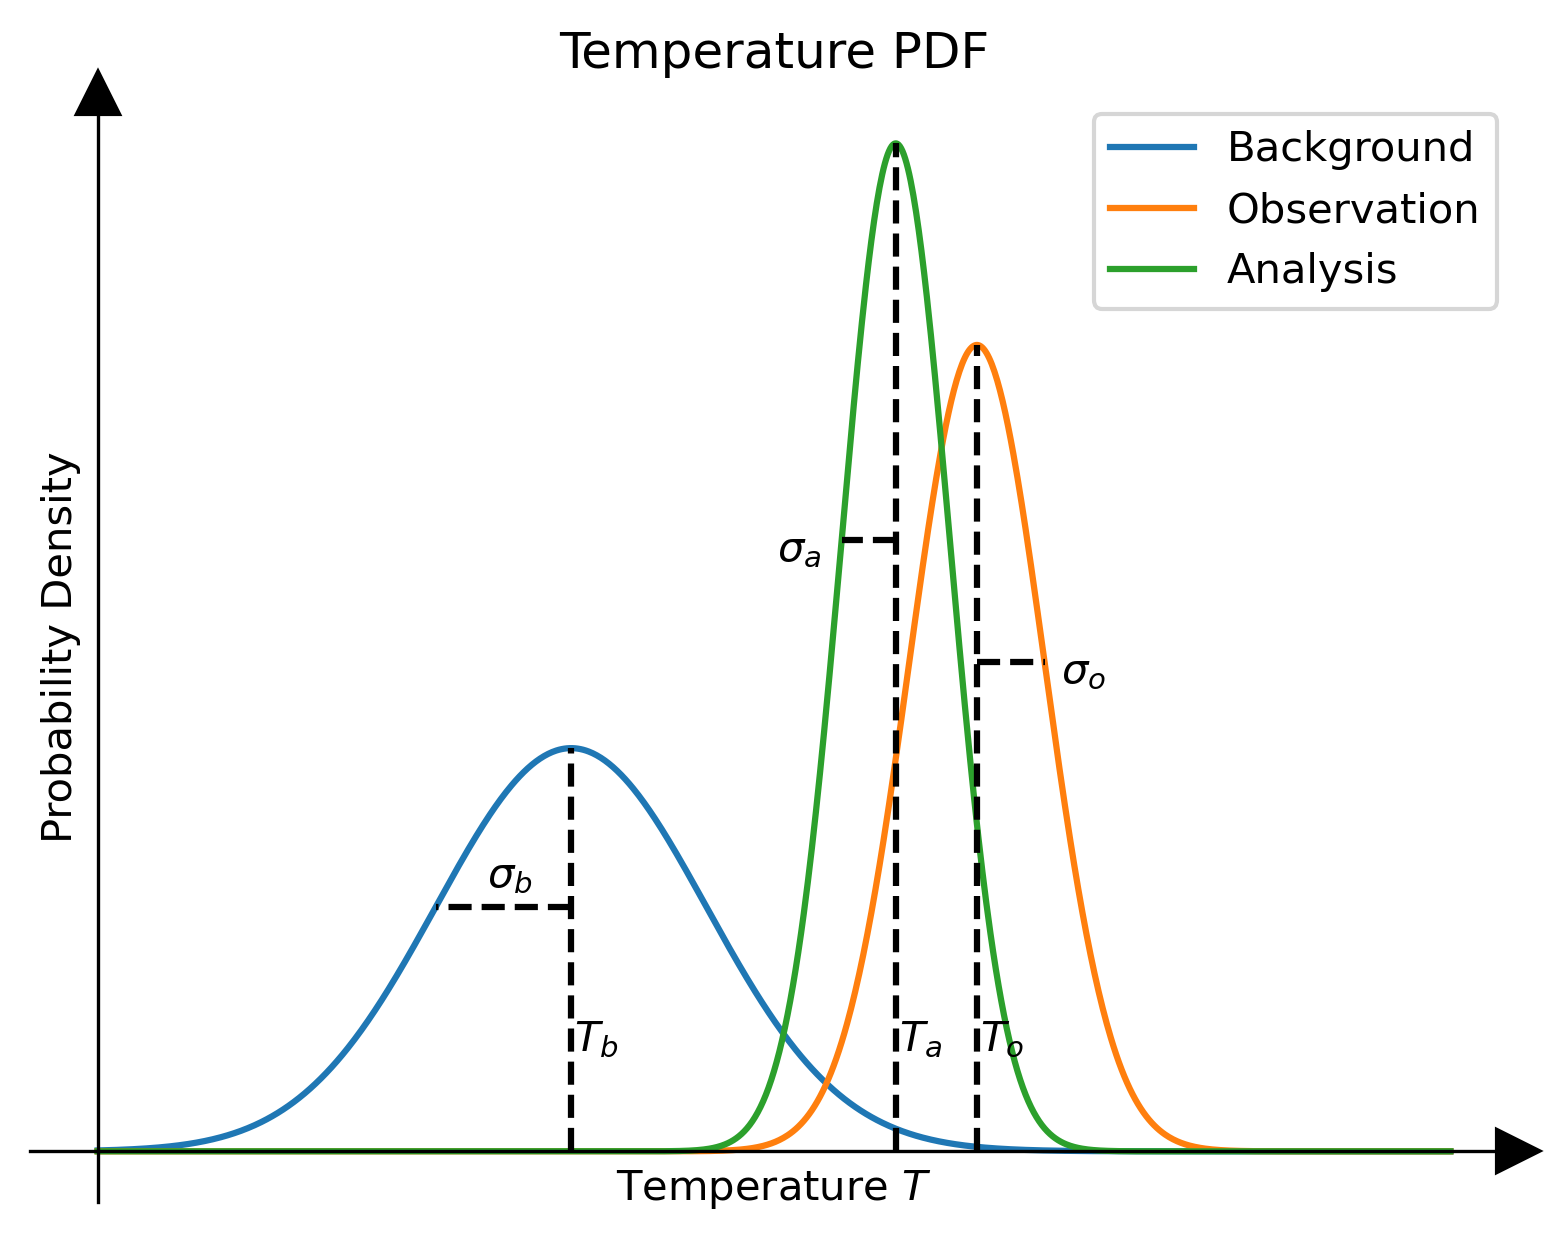
\includegraphics[scale=0.75]{graphics/DA1.png}
    \caption{The probability density distribution of the background/observation/analysis temperatures in the section example where the errors are assumed to have a Gaussian shape.}
    \label{fig:DA1}
\end{figure}

\subsection{Optimal Interpolation}

In the last subsection, we only use a single variable as the illustrating example. Obviously, in actual weather models, there will be multiple variables (let's say $N$) like temperature, pressure, density, and three-dimensional winds to be simulated in a large number of grid points ($M$). Hence there will be a total of $L = MN$ variables in the model output and we will place all of them into a \textit{state vector} of length $L = MN$:
\begin{align}
\textbf{x} = 
\begin{bmatrix}
x_1 \\
x_2 \\
\vdots \\
x_L
\end{bmatrix}
\end{align}
with a corresponding error vector of
\begin{align}
\bm{\epsilon} =  
\begin{bmatrix}
\varepsilon_1 \\
\varepsilon_2 \\
\vdots \\
\varepsilon_L
\end{bmatrix}
\end{align}
which is assumed to be unbiased too, such that the expected values of the errors $E(\bm{\epsilon}) = \textbf{0}$ is always a zero vector. The \textit{error covariance matrix} is then defined as
\begin{align}
P &= E[(\bm{\epsilon} - E(\bm{\epsilon}))(\bm{\epsilon} - E(\bm{\epsilon}))^T] = E[\bm{\epsilon}\bm{\epsilon}^T] \nonumber \\
&= \begin{bmatrix}
E[\varepsilon_1\varepsilon_1] & E[\varepsilon_1\varepsilon_2] & \cdots & E[\varepsilon_1\varepsilon_L] \\
E[\varepsilon_2\varepsilon_1] & E[\varepsilon_2\varepsilon_2] & & E[\varepsilon_1\varepsilon_L] \\
\vdots & & \ddots & \vdots \\
E[\varepsilon_L\varepsilon_1] & E[\varepsilon_L\varepsilon_2] & \cdots & E[\varepsilon_L\varepsilon_L] 
\end{bmatrix}
\end{align}
which is generalized from Properties \ref{proper:variancemul}. We will start with the simplest case where the observations are exactly the model variables. Then the background, analysis, and observation states can be expressed as
\begin{subequations}
\label{eqn:OIxbaoe}
\begin{align}
\textbf{x}_b = \textbf{x}_t + \bm{\epsilon}_b \\
\textbf{x}_a = \textbf{x}_t + \bm{\epsilon}_a \\
\textbf{x}_o = \textbf{x}_t + \bm{\epsilon}_o
\end{align}    
\end{subequations}
relative to the truth $\textbf{x}_t$. The error covariance matrices for the background, analysis, and observation are
\begin{subequations}
\label{eqn:OIPmat}
\begin{align}
P_b &= B = E[\bm{\epsilon}_b\bm{\epsilon}_b^T] \\
P_a &= A = E[\bm{\epsilon}_a\bm{\epsilon}_a^T] \\
P_o &= R = E[\bm{\epsilon}_o\bm{\epsilon}_o^T]
\end{align}    
\end{subequations}
As before, we assume that the background and observation errors are uncorrelated so that
\begin{align}
E[\bm{\epsilon}_b\bm{\epsilon}_o^T] = E[\bm{\epsilon}_o\bm{\epsilon}_b^T] = \textbf{0} \label{eqn:OIuncorr}
\end{align}
We also require the analysis $\textbf{x}_a$ to be an unbiased linear combination of $\textbf{x}_b$ and $\textbf{x}_o$. This allows us to write
\begin{align}
\textbf{x}_a &= \textbf{x}_b + K(\textbf{x}_o - \textbf{x}_b)  \label{eqn:OIinnov}
\end{align}
akin to (\ref{eqn:uniDAweight}) where $K$ is the \textit{Kalman gain} matrix that represents the optimal weight. Therefore, the analysis will be the background plus the optimal weight times the observation increment (\textit{innovation}). Subsequently,
\begin{align}
\textbf{x}_t + \bm{\epsilon}_a &= \textbf{x}_t + \bm{\epsilon}_b + K(\textbf{x}_o - \textbf{x}_t - \bm{\epsilon}_b) \nonumber \\
\bm{\epsilon}_a &= \bm{\epsilon}_b + K(\bm{\epsilon}_o - \bm{\epsilon}_b) \label{eqn:varakalman}
\end{align}
The total error variance $E[\bm{\epsilon}_a^T\bm{\epsilon}_a]$, or equivalently the trace of $A$, by Index Notation, is
\begin{align}
E[\bm{\epsilon}_a^T\bm{\epsilon}_a] = E[(\varepsilon_a)_i(\varepsilon_a)_i)]  
\end{align}
Similar to (\ref{eqn:DAunimin}), we want to differentiate this quantity but with respect to the Kalman gain matrix $K$ and demand that
\begin{align}
\frac{\partial E[\bm{\epsilon}_a^T\bm{\epsilon}_a]}{\partial K} = E\left(\frac{\partial [\bm{\epsilon}_a^T\bm{\epsilon}_a]}{\partial K}\right) = [\textbf{0}] \label{eqn:Kalmande0}
\end{align}
To proceed, we first note that it works very much like (\ref{eqn:dxdxdelta}) but with two Kronecker deltas now:
\begin{align}
\frac{\partial K_{ij}}{\partial K_{pq}} = \delta_{ip}\delta_{jq}
\end{align}
Now, writing out the subscripts in (\ref{eqn:varakalman}), we have
\begin{align}
(\varepsilon_a)_i(\varepsilon_a)_i = [(\varepsilon_b)_i + K_{ij}((\varepsilon_o)_j - (\varepsilon_b)_j)][(\varepsilon_b)_i + K_{ik}((\varepsilon_o)_k - (\varepsilon_b)_k)]
\end{align}
where we have to use two different dummy indices for the product due to the rule of Index Notation. Then the derivative is computed to be
\begin{align}
&\quad \frac{\partial [\bm{\epsilon}_a^T\bm{\epsilon}_a]}{\partial K} \nonumber \\
&= \frac{\partial}{\partial K_{pq}}\left([(\varepsilon_b)_i + K_{ij}((\varepsilon_o)_j - (\varepsilon_b)_j)][(\varepsilon_b)_i + K_{ik}((\varepsilon_o)_k - (\varepsilon_b)_k)]\right) \nonumber \\
&= \left(\frac{\partial}{\partial K_{pq}}[(\varepsilon_b)_i + K_{ij}((\varepsilon_o)_j - (\varepsilon_b)_j)]\right)[(\varepsilon_b)_i + K_{ik}((\varepsilon_o)_k - (\varepsilon_b)_k)] \nonumber \\
&\quad +[(\varepsilon_b)_i + K_{ij}((\varepsilon_o)_j - (\varepsilon_b)_j)] \left(\frac{\partial}{\partial K_{pq}}[(\varepsilon_b)_i + K_{ik}((\varepsilon_o)_k - (\varepsilon_b)_k)]\right) \nonumber \\
&= \delta_{ip}\delta_{jq}((\varepsilon_o)_j - (\varepsilon_b)_j)[(\varepsilon_b)_i + K_{ik}((\varepsilon_o)_k - (\varepsilon_b)_k)] \nonumber \\
&\quad + ((\varepsilon_b)_i + K_{ij}((\varepsilon_o)_j - (\varepsilon_b)_j)) \delta_{ip}\delta_{kq} ((\varepsilon_o)_k - (\varepsilon_b)_k) \nonumber \\
&= ((\varepsilon_o)_q - (\varepsilon_b)_q)[(\varepsilon_b)_p + K_{pk}((\varepsilon_o)_k - (\varepsilon_b)_k)] \nonumber \\
&\quad + ((\varepsilon_b)_p + K_{pj}((\varepsilon_o)_j - (\varepsilon_b)_j)) ((\varepsilon_o)_q - (\varepsilon_b)_q) \nonumber \\
&= 2((\varepsilon_b)_p + K_{pk}((\varepsilon_o)_k - (\varepsilon_b)_k)) ((\varepsilon_o)_q - (\varepsilon_b)_q) \nonumber \\
&\quad \text{(One of the dummy indices can be changed and the terms will be grouped)} \nonumber \\
&= 2(\varepsilon_b)_p ((\varepsilon_o)_q - (\varepsilon_b)_q) + 2 K_{pk}((\varepsilon_o)_k - (\varepsilon_b)_k)((\varepsilon_o)_q - (\varepsilon_b)_q) \nonumber \\
&= 2 \bm{\epsilon}_b (\bm{\epsilon}_o - \bm{\epsilon}_b)^T + 2K(\bm{\epsilon}_o - \bm{\epsilon}_b)(\bm{\epsilon}_o - \bm{\epsilon}_b)^T \label{eqn:Kalmande0res}
\end{align}
where in the last step we convert it back to matrix form. Plugging it into (\ref{eqn:Kalmande0}) gives the desired expression for the Kalman gain matrix.
\begin{align}
E\left(\frac{\partial [\bm{\epsilon}_a^T\bm{\epsilon}_a]}{\partial K}\right) = E[2 \bm{\epsilon}_b (\bm{\epsilon}_o - \bm{\epsilon}_b)^T + 2K(\bm{\epsilon}_o - \bm{\epsilon}_b)(\bm{\epsilon}_o - \bm{\epsilon}_b)^T] &= [\textbf{0}] \nonumber \\
E[\bm{\epsilon}_b\bm{\epsilon}_o^T] - E[\bm{\epsilon}_b\bm{\epsilon}_b^T] + K(E[\bm{\epsilon}_o\bm{\epsilon}_o^T] - E[\bm{\epsilon}_b\bm{\epsilon}_o^T] - E[\bm{\epsilon}_o\bm{\epsilon}_b^T] + E[\bm{\epsilon}_b\bm{\epsilon}_b^T)] &= [\textbf{0}] \nonumber \\
- E[\bm{\epsilon}_b\bm{\epsilon}_b^T] + K(E[\bm{\epsilon}_o\bm{\epsilon}_o^T] + E[\bm{\epsilon}_b\bm{\epsilon}_b^T]) &= [\textbf{0}] \nonumber \\
\text{(Uncorrelated errors by (\ref{eqn:OIuncorr}))} & \nonumber \\
- B + K(B+R) &= [\textbf{0}] \nonumber \\
\implies K = B(B+R)&^{-1} \label{eqn:OImatK}
\end{align}
The analysis covariance is
\begin{align}
A &= E[\bm{\epsilon}_a\bm{\epsilon}_a^T] \nonumber \\
&= E[(\bm{\epsilon}_b + K(\bm{\epsilon}_o - \bm{\epsilon}_b))(\bm{\epsilon}_b + K(\bm{\epsilon}_o - \bm{\epsilon}_b))^T] \nonumber \\
&= E[\bm{\epsilon}_b\bm{\epsilon}_b^T] + E[\bm{\epsilon}_bK(\bm{\epsilon}_o - \bm{\epsilon}_b)^T] \nonumber \\
&\quad + E[K(\bm{\epsilon}_o - \bm{\epsilon}_b)\bm{\epsilon}_b^T] + E[K(\bm{\epsilon}_o - \bm{\epsilon}_b)(K(\bm{\epsilon}_o - \bm{\epsilon}_b))^T] \nonumber \\
&= E[\bm{\epsilon}_b\bm{\epsilon}_b^T] + E[\bm{\epsilon}_b(\bm{\epsilon}_o - \bm{\epsilon}_b)^TK^T] \nonumber \\
&\quad + E[K(\bm{\epsilon}_o - \bm{\epsilon}_b)\bm{\epsilon}_b^T] + E[K(\bm{\epsilon}_o - \bm{\epsilon}_b) (\bm{\epsilon}_o - \bm{\epsilon}_b)^TK^T] \nonumber \\
&= B - BK^T - KB + K(B+R)K^T \qquad \text{(Uncorrelated errors by (\ref{eqn:OIuncorr}))} \nonumber \\
&= B - BK^T - KB + B(B+R)^{-1} (B+R)K^T \qquad \text{(by (\ref{eqn:OImatK}))} \nonumber \\
&= B - BK^T - KB + BK^T = B - KB = (I-K)B \label{eqn:OIAnalysis}
\end{align}
(\ref{eqn:OIinnov}), (\ref{eqn:OImatK}), and (\ref{eqn:OIAnalysis}) then constitute the \textit{multivariate} \index{Optimal Interpolation}\keywordhl{Optimal Interpolation} scheme that can be compared to (\ref{eqn:univOIschm}). An alternative form for $K$ and $A$ can be derived as follows.
\begin{align}
K = B(B+R)^{-1} &= B[(RR^{-1})B+R(B^{-1}B)]^{-1} \nonumber \\
&= B[R(R^{-1} + B^{-1})B]^{-1} \nonumber  \\
&= BB^{-1}(B^{-1} + R^{-1})^{-1}R^{-1} = (B^{-1} + R^{-1})^{-1}R^{-1} \label{eqn:OIKalt}
\end{align}
\begin{align}
A = B - KB &= B - (B^{-1} + R^{-1})^{-1}R^{-1} B \nonumber \\
&= (B^{-1} + R^{-1})^{-1}(B^{-1} + R^{-1})B - (B^{-1} + R^{-1})^{-1} R^{-1} B \nonumber \\
&= (B^{-1} + R^{-1})^{-1} ((B^{-1} + R^{-1})B - R^{-1} B) \nonumber \\
&= (B^{-1} + R^{-1})^{-1} (B^{-1}B + R^{-1}B - R^{-1} B) \nonumber \\
&= (B^{-1} + R^{-1})^{-1} I = (B^{-1} + R^{-1})^{-1} \nonumber \\
\implies A^{-1} &= B^{-1} + R^{-1}
\end{align}
Same as the univariate case, the inverses of covariance matrices represent the precisions and the analysis precision is just the sum of those of the background and observation. \par

However, most of the time, the observations are not exactly the model variables or measured at different locations from the grid points. Let there be $G$ observations stored in a vector $\textbf{y}_o$, and it is related to the model variables by the observation operator $H$ according to $\textbf{y} = H(\textbf{x})$. Then (a) and (b) of (\ref{eqn:OIxbaoe}) remain the same but (c) is now 
\begin{align}
\textbf{y}_o = H(\textbf{x}_t) + \bm{\epsilon}_o \label{eqn:OIinnover}
\end{align}
where $\textbf{y}_o$ and $ \bm{\epsilon}_o$ are vectors of length $G$. Due to the scope limit, we will only discuss the case where the observation operator $H$ is linear and hence a matrix such that
\begin{align}
\textbf{y} = H(\textbf{x}) = H\textbf{x}   
\end{align}
Then the innovation vector will be 
\begin{align}
\textbf{d} &= \textbf{y}_o - H\textbf{x}_b \nonumber \\
&= \textbf{y}_o - H(\textbf{x}_t + \bm{\epsilon}_b) \nonumber \\
&= \textbf{y}_o - H\textbf{x}_t - H\bm{\epsilon}_b \nonumber \\
&= \bm{\epsilon}_o -  H\bm{\epsilon}_b
\end{align}
Similar to the previous formulation, we compute the analysis as the background plus the optimal weight times the innovation:
\begin{align}
\textbf{x}_a &= \textbf{x}_b + K(\textbf{y}_o - H\textbf{x}_b) = \textbf{x}_b + K\textbf{d} \label{eqn:OIinnov1} \\
\textbf{x}_t + \bm{\epsilon}_a &= \textbf{x}_t + \bm{\epsilon}_b + K\textbf{d} \implies \bm{\epsilon}_a = \bm{\epsilon}_b + K\textbf{d} 
\end{align}
We demand the same as in (\ref{eqn:Kalmande0}). However, note that the only difference of the above expression from (\ref{eqn:varakalman}) is that $\textbf{x}_o - \textbf{x}_b$ is replaced by $\textbf{d}$ and (\ref{eqn:Kalmande0res}) simply becomes
\begin{align}
\frac{\partial (\bm{\epsilon}_a^T\bm{\epsilon}_a)}{\partial K} = 2\bm{\epsilon}_b\textbf{d}^T + 2K\textbf{d}\textbf{d}^T
\end{align}
As before, we require the expected value of this derivative to be zero, and hence
\begin{align}
\frac{\partial E[\bm{\epsilon}_a^T\bm{\epsilon}_a]}{\partial K} = E[2\bm{\epsilon}_b\textbf{d}^T + 2K\textbf{d}\textbf{d}^T] &= [\textbf{0}] \nonumber \\
E[\bm{\epsilon}_b(\bm{\epsilon}_o -  H\bm{\epsilon}_b)^T + K(\bm{\epsilon}_o -  H\bm{\epsilon}_b)(\bm{\epsilon}_o -  H\bm{\epsilon}_b)^T] &= [\textbf{0}] \nonumber \\
E[\bm{\epsilon}_b\bm{\epsilon}_b^TH^T] + KE[\bm{\epsilon}_o\bm{\epsilon}_o^T] + KE[H\bm{\epsilon}_b\bm{\epsilon}_b^TH^T] &= [\textbf{0}] \nonumber \\ 
 \text{(Uncorrelated errors by (\ref{eqn:OIuncorr}))} & \nonumber \\
-BH^T + K(R+HBH^T) &= [\textbf{0}] \nonumber \\
\implies K &= BH^T(HBH^T+R)^{-1} \label{eqn:OImatK2}
\end{align}
The analysis covariance is now
\begin{align}
A &= E[\bm{\epsilon}_a\bm{\epsilon}_a^T] \nonumber \\
&= E[(\bm{\epsilon}_b + K(\bm{\epsilon}_o - H\bm{\epsilon}_b))(\bm{\epsilon}_b + K(\bm{\epsilon}_o - H\bm{\epsilon}_b))^T] \nonumber \\
&= E[\bm{\epsilon}_b\bm{\epsilon}_b^T] - E[KH\bm{\epsilon}_b\bm{\epsilon}_b^T] - E[\bm{\epsilon}_b(KH\bm{\epsilon}_b)^T] \nonumber \\
&\quad + E[(K\bm{\epsilon}_o)(K\bm{\epsilon}_o)^T] + E[KH\bm{\epsilon}_b(KH\bm{\epsilon}_b)^T] \nonumber \\
&\quad \text{(Uncorrelated errors by (\ref{eqn:OIuncorr}))} \nonumber \\
&= E[\bm{\epsilon}_b\bm{\epsilon}_b^T] - E[KH\bm{\epsilon}_b\bm{\epsilon}_b^T] - E[\bm{\epsilon}_b\bm{\epsilon}_b^TH^TK^T] \nonumber \\
&\quad + E[K\bm{\epsilon}_o\bm{\epsilon}_o^TK^T] + E[KH\bm{\epsilon}_b\bm{\epsilon}_b^TH^TK^T] \nonumber \\
&= B - KHB - BH^TK^T + KRK^T + KHBH^TK^T \nonumber \\
&= B - KHB - BH^TK^T + K(HBH^T+R)K^T \nonumber \\
&= B - KHB - BH^TK^T + BH^T(HBH^T+R)^{-1}(HBH^T+R)K^T &\text{(by (\ref{eqn:OImatK2}))} \nonumber \\
&= B - KHB - BH^TK^T + BH^TK^T \nonumber \\
&= B - KHB = (I-KH)B \label{eqn:OIcovA}
\end{align}
Similar to (\ref{eqn:OIKalt}), we can express $K$ in an alternative form. We may be tempted to write 
\begin{align*}
K &= BH^T(HBH^T+R)^{-1} \\
&= BH^T[(H^TR^{-1})^{-1}(H^TR^{-1})HBH^T+R(BH^T)^{-1}(BH^T)]^{-1} 
\end{align*}
just like (\ref{eqn:OIKalt}). However, $H$ will be a non-square $G \times L$ matrix, hence $H^TR^{-1}$ and $BH^T$ are also not square, and their inverses are not defined. To proceed, we need the \index{Sherman-Morrison-Woodbury Formula}\keywordhl{Sherman-Morrison-Woodbury Formula}:
\begin{align}
(A + SXC)^{-1} = A^{-1} - A^{-1}S(X^{-1} + CA^{-1}S)^{-1}CA^{-1}
\end{align}
This can be derived by comparing the upper-left block of Properties \ref{proper:schurinv} and \ref{proper:schurinvD} with $D$ replaced by $-X^{-1}$ and $B$ replaced by $S$. Now substitute $A = R$, $S = H$, $X = B$, $C=H^T$ to get
\begin{align}
(HBH^T + R)^{-1} = R^{-1} - R^{-1}H(B^{-1} + H^TR^{-1}H)^{-1}H^T R^{-1}    
\end{align}
Plugging it into (\ref{eqn:OImatK2}), we have
\begin{align}
K &= BH^T(HBH^T+R)^{-1} \nonumber \\
&= BH^T(R^{-1} - R^{-1}H(B^{-1} + H^TR^{-1}H)^{-1}H^T R^{-1}) \nonumber \\
&= BH^TR^{-1} - BH^TR^{-1}H(B^{-1} + H^TR^{-1}H)^{-1}H^T R^{-1} \nonumber \\
&= B(B^{-1} + H^TR^{-1}H)(B^{-1} + H^TR^{-1}H)^{-1}H^TR^{-1} \nonumber \\
&\quad- BH^TR^{-1}H(B^{-1} + H^TR^{-1}H)^{-1}H^T R^{-1} \nonumber \\
&= (B(B^{-1} + H^TR^{-1}H) - BH^TR^{-1}H)(B^{-1} + H^TR^{-1}H)^{-1}H^TR^{-1} \nonumber \\
&= (BB^{-1} + BH^TR^{-1}H - BH^TR^{-1}H)(B^{-1} + H^TR^{-1}H)^{-1}H^TR^{-1} \nonumber \\
&= I(B^{-1} + H^TR^{-1}H)^{-1}H^TR^{-1} = (B^{-1} + H^TR^{-1}H)^{-1}H^TR^{-1}
\end{align}
and the analysis covariance can be rewritten as
\begin{align}
A = B - KHB &= B - (B^{-1} + H^TR^{-1}H)^{-1}H^TR^{-1}HB \nonumber \\
&= (B^{-1} + H^TR^{-1}H)^{-1}(B^{-1} + H^TR^{-1}H)B \nonumber \\
&\quad- (B^{-1} + H^TR^{-1}H)^{-1}H^TR^{-1}HB \nonumber \\
&= (B^{-1} + H^TR^{-1}H)^{-1}((B^{-1} + H^TR^{-1}H)B - H^TR^{-1}HB) \nonumber \\
&= (B^{-1} + H^TR^{-1}H)^{-1}(B^{-1}B + H^TR^{-1}HB - H^TR^{-1}HB) \nonumber \\
&= (B^{-1} + H^TR^{-1}H)^{-1} \implies A^{-1} = B^{-1} + H^TR^{-1}H
\end{align}

\subsection{Kalman Filter}

Notice that the technique of Optimal Interpolation introduced in the last subsection does not depend on time and can be used at any time step in an isolated fashion. However, in physical models, we need to integrate forwards in time for the forecast. We may ask if there is an improved version of Optimal Interpolation such that it will take the evolution of the model state into account. Particularly, the background error is previously assumed to be static but should actually change in time, e.g. different climatologies in different seasons. \index{Kalman Filter}\keywordhl{Kalman Filter} solves this by further cycling the background error covariance using the model. It is essentially Optimal Interpolation but with the error covariances evolved forward in time as well. No matter how the background error is initially determined, it will become more and more optimal after several cycles as long as the model and observations are good. Kalman Filter consists of two steps: the \textit{analysis step} which is identical to Optimal Interpolation, and the \textit{forecast step} where we carry out time integration for the state vector and the error covariance matrix in the model.\par

In Kalman filter, a short-term model forecast is used as the background and the subscript $b$ is now replaced by $f$, and similar to (\ref{eqn:OIxbaoe}) plus (\ref{eqn:OIinnover}), we have
\begin{subequations}
\begin{align}
\textbf{x}_f^{[i]} = \textbf{x}_t^{[i]} + \bm{\epsilon}_f^{[i]} \\
\textbf{x}_a^{[i]} = \textbf{x}_t^{[i]} + \bm{\epsilon}_a^{[i]} \\
\textbf{y}_o^{[i]} = H\textbf{x}_t^{[i]} + \bm{\epsilon}_o^{[i]}    
\end{align}    
\end{subequations}
where the superscript $^{[i]}$ indicates the $i$-th time step. Also (\ref{eqn:OIPmat}) is now
\begin{subequations}
\begin{align}
P_f^{[i]} &= E[\bm{\epsilon}_f^{[i]}\bm{\epsilon}_f^{[i]T}] \\
P_a^{[i]} &= E[\bm{\epsilon}_a^{[i]}\bm{\epsilon}_a^{[i]T}] \\
R^{[i]} &= E[\bm{\epsilon}_o^{[i]}\bm{\epsilon}_o^{[i]T}]    
\end{align}
\end{subequations}
The forward integration model $M$ is assumed to be linear such that the forecast at the next time step is given by
\begin{subequations}
\label{eqn:forecastKalman}
\begin{align}
\textbf{x}_f^{[i+1]} &= M^{[i]}\textbf{x}_a^{[i]} \label{eqn:xaMxf} \\
\textbf{x}_t^{[i+1]} &= M^{[i]}\textbf{x}_t^{[i]} - \bm{\eta}^{[i]}
\end{align}
\end{subequations}
where $M^{[i]}$ is the corresponding forward mapping at the $i$-th time step and $\bm{\eta}^{[i]}$ represents the inherent model error vector. We assume that
\begin{subequations}
\begin{align}
E[\bm{\eta}^{[i]}] &= \textbf{0} \\
E[\bm{\epsilon}_a^{[i]}\bm{\eta}^{[i]T}] = E[\bm{\eta}_a^{[i]}\bm{\epsilon}^{[i]T}] &= [\textbf{0}] \label{eqn:modelanluncorr}\\
Q^{[i]} &= E[\bm{\eta}^{[i]}\bm{\eta}^{[i]T}]
\end{align}   
\end{subequations}
the model error is unbiased and uncorrelated to that of the analysis, with an error covariance matrix of $Q$. As said before, the analysis step remains identical, and (\ref{eqn:OIinnov1}), (\ref{eqn:OImatK2}), (\ref{eqn:OIcovA}) will be the same except the matrices are now differently denoted:
\begin{subequations}
\begin{align}
\textbf{x}_a^{[i]} &= \textbf{x}_f^{[i]} + K^{[i]}(\textbf{y}_o^{[i]} - H\textbf{x}_f^{[i]}) \\
K^{[i]} &= P_f^{[i]}H^T(HP_f^{[i]}H^T + R^{[i]})^{-1} \\
P_a^{[i]} &= (I - K^{[i]}H)P_f^{[i]} 
\end{align}
\end{subequations}
Meanwhile, the forecast equations are (\ref{eqn:xaMxf}) for the model state, and for the error covariance, we have
\begin{align}
\bm{\epsilon}_f^{[i+1]} &= \textbf{x}_f^{[i+1]} - \textbf{x}_t^{[i+1]} \nonumber \\
&= M^{[i]}\textbf{x}_a^{[i]} - (M^{[i]}\textbf{x}_t^{[i]} - \bm{\eta}^{[i]}) &\text{(by (\ref{eqn:forecastKalman}))} \nonumber \\
&= M^{[i]}(\textbf{x}_a^{[i]} - \textbf{x}_t^{[i]}) + \bm{\eta}^{[i]} \nonumber \\
&= M^{[i]}\bm{\epsilon}_a^{[i]} + \bm{\eta}^{[i]}  
\end{align}
and thus
\begin{align}
P_f^{[i+1]} &= E[\bm{\epsilon}_f^{[i+1]}\bm{\epsilon}_f^{[i+1]T}] \nonumber \\
&= E[(M^{[i]}\bm{\epsilon}_a^{[i]} + \bm{\eta}^{[i]})(M^{[i]}\bm{\epsilon}_a^{[i]} + \bm{\eta}^{[i]})^T] \nonumber \\
&= M^{[i]}E[\bm{\epsilon}_a^{[i]}\bm{\epsilon}_a^{[i]T}]M^{[i]T} + E[\bm{\eta}^{[i]}\bm{\eta}^{[i]T}] &\text{(by (\ref{eqn:modelanluncorr}))} \nonumber \\
&= M^{[i]}P_a^{[i]}M^{[i]T} + Q^{[i]} \label{eqn:MPMQ}
\end{align}
The forecast step then consists of (\ref{eqn:xaMxf}) and (\ref{eqn:MPMQ}). There are two ways to implement Kalman Filter. The standard scheme is to compute the Kalman gain first in the analysis step while the other scheme is to the analysis error covariance first. The flowcharts for these two implementations are shown in Figures \ref{fig:Kalmansteps} and \ref{fig:Kalmansteps2}.

\begin{landscape}
\begin{figure}
    \centering
    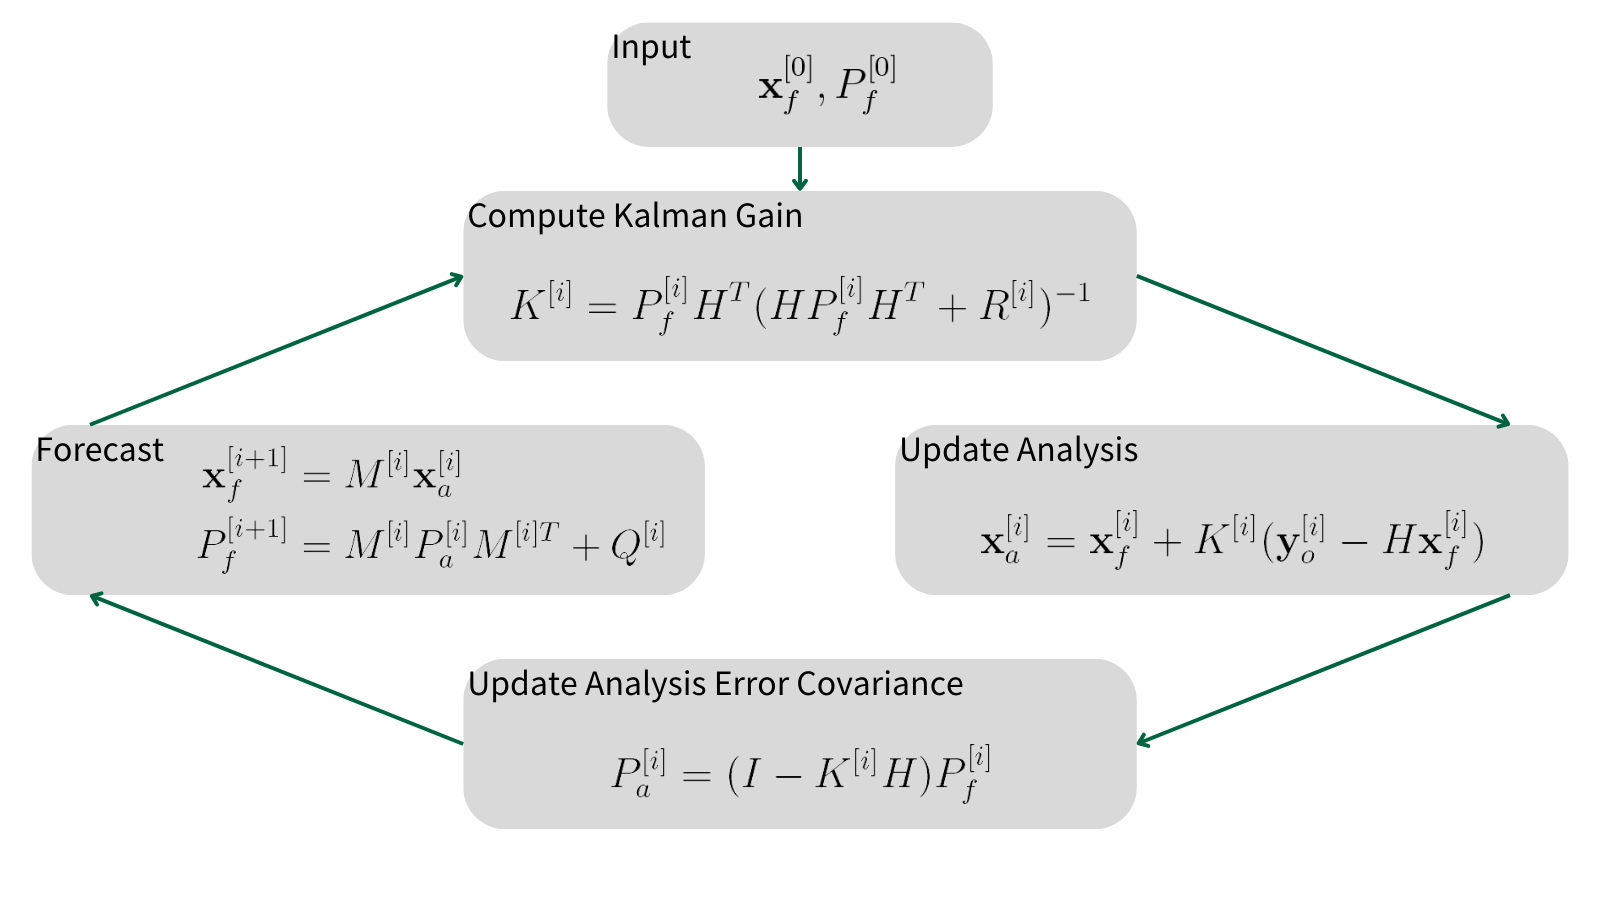
\includegraphics[width=0.99\linewidth]{graphics/Kalman1.png}
    \caption{The flowchart for the standard Kalman Filter scheme.}
    \label{fig:Kalmansteps}
\end{figure}
\end{landscape}
\begin{landscape}
\begin{figure}
    \centering
    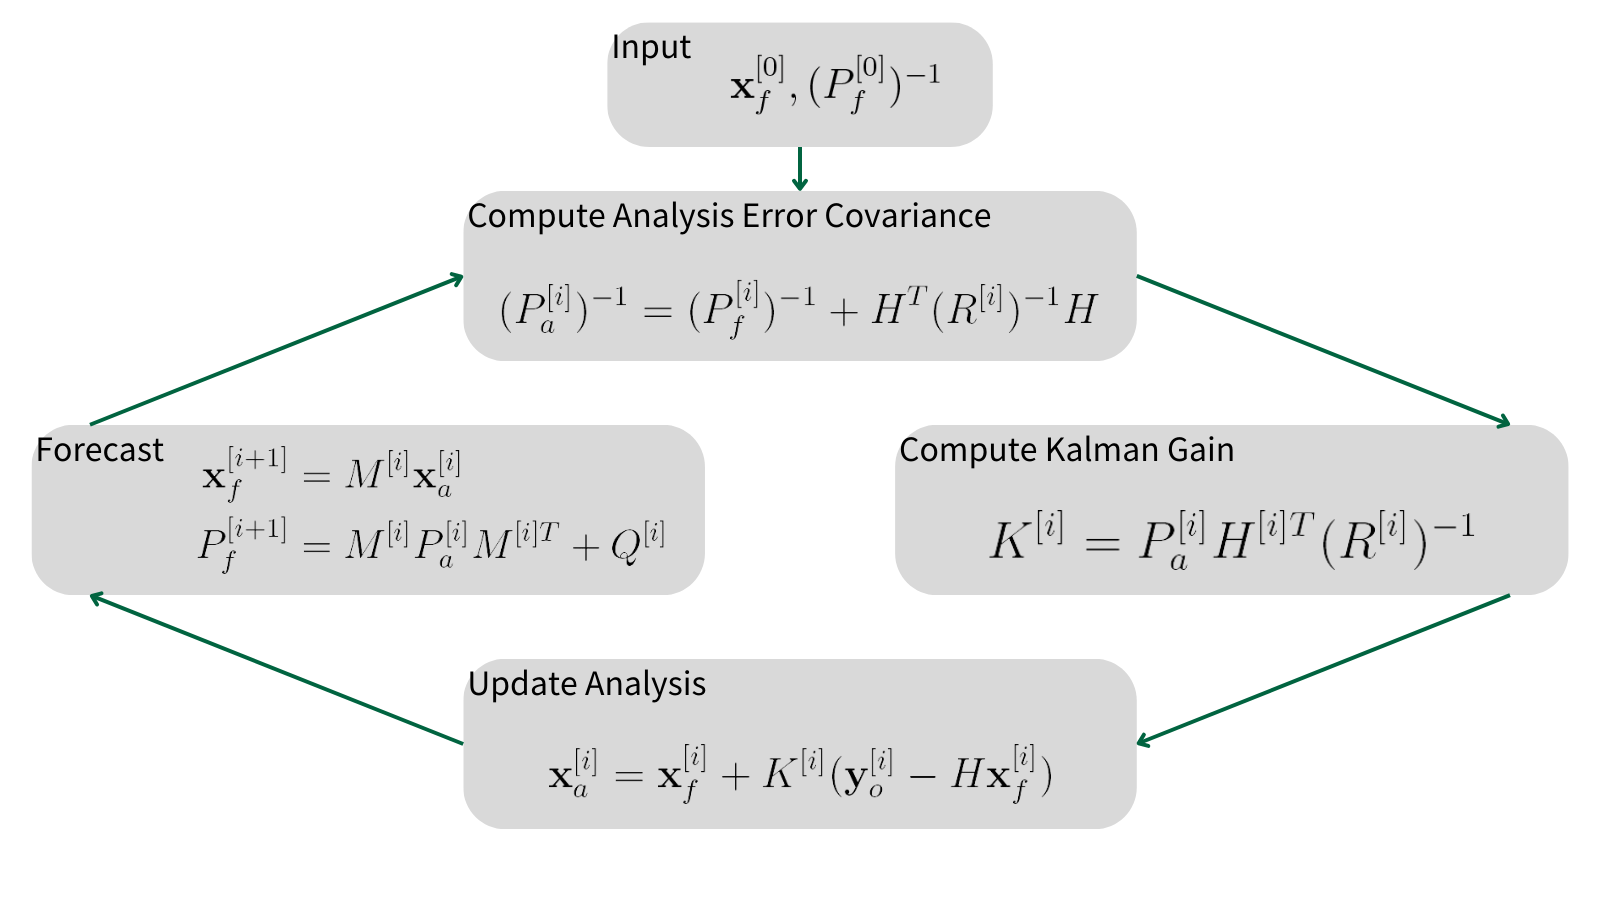
\includegraphics[width=0.99\linewidth]{graphics/Kalman2.png}
    \caption{The flowchart for the alternative Kalman Filter scheme using equivalent expressions for the analysis error covariance and Kalman gain.}
    \label{fig:Kalmansteps2}
\end{figure}
\end{landscape}

\subsection{Python Programming: Demonstration of DA using the Lorenz-63 Model}
\label{subsection:DAsystem}

We will use the Lorenz-63 Model to demonstrate the implementation of Kalman Filter. First, borrow the codes from the last chapter to create a ground truth for the evolution of the Lorenz-63 system.
\begin{lstlisting}
import matplotlib.pyplot as plt
import numpy as np
from scipy.integrate import solve_ivp

def Lorenz63(t, y, sigma=10, beta=8/3, rho=28):
    X, Y, Z = y[0], y[1], y[2]
    dXdt = -sigma*X + sigma*Y
    dYdt = -X*Z + rho*X - Y
    dZdt = X*Y - beta*Z
    return([dXdt, dYdt, dZdt])

t_span = [0,5]
dt = 0.01
x_0 = [-4,10,8]

sol_t = solve_ivp(Lorenz63, t_span, x_0, t_eval=np.arange(t_span[0], t_span[1], dt))
x_t = sol_t.y.T
\end{lstlisting}
From this, we also generate a time-series of synthetic observations by adding Gaussian noises with a constant error covariance of $R = 0.5I$.
\begin{lstlisting}
R = np.diag([0.5]*3)
obs_errors = np.random.multivariate_normal([0,0,0], R, x_t.shape[0])
x_o = x_t + obs_errors    
\end{lstlisting}
Since the Lorenz-63 system is non-linear, for the algorithm of Kalman Filter to work properly, we have to use the \textit{Tangent Linear Model} in place of $M^{[i]}$ when computing $P_f^{[i]}$:
\begin{align}
M^{[i]} = I + (\frac{\partial F}{\partial \textbf{x}})_a^{[i]} \Delta t
\end{align}
where $\partial F/\partial \textbf{x}$ is the Jacobian of the Lorenz-63 system as in (\ref{eqn:lorenzjac}). We will integrate the model forward in time using the simple \textit{Euler method} at the forecast step. On the other hand, at the analysis step, we have to compute the Kalman gain and analysis (as well as its error covariance). To initialize, we will make a guess of \smash{$P_f^{[0]} = 0.5I$}, which is not a problem as the Kalman Filter procedure itself will cycle and tune the error covariance. Finally, we simply have $H = I$ as we will use the synthetic observations of all exact variables. The final program will look like this:
\begin{lstlisting}
sigma, beta, rho = 10, 8/3, 28
P_f_i = np.diag([0.5]*3)
H = np.identity(3)
x_a = np.array([[-5,12,6]]) # Assume some initial error
x_f_i = x_a[0,:]

for ii in np.arange(x_t.shape[0]):

    Ts = ii*dt # Forecast start time
    Ta = (ii+1)*dt # Forecast end time (DA analysis time)

    #--------------
    # Analysis Step
    #--------------

    K_i = P_f_i @ H.T @ np.linalg.inv(H @ P_f_i @ H.T + R) # Compute Kalman gain

    d = x_o[ii, :] - H @ x_f_i # Innovation
    x_a_i = x_f_i + K_i @ d # Update analysis
    P_a_i = (np.identity(3) - K_i @ H) @ P_f_i # plus its error covariance
    
    if ii >= 1:
        x_a = np.vstack([x_a, [x_a_i]]) # Save the analysis output

    #--------------
    # Forecast Step
    #--------------
    
    x_f_i = x_a_i + np.array(Lorenz63(Ts, x_a_i))*dt # Forecast by Euler
    Jcb = np.array([[-sigma,       sigma,    0        ],
                    [rho-x_f_i[2], -1,       -x_f_i[0]],
                    [x_f_i[1],     x_f_i[0], -beta    ]]) # Jacobian
    M_i = np.identity(3) + Jcb*dt # Tangent Linear Model
    P_f_i = M_i @ P_a_i @ M_i.T + np.diag([0.1]*3) # Assume Q = 0.1I
\end{lstlisting}
Let's visualize the performance of our DA system by looking at the errors:
\begin{lstlisting}
err = np.sum(np.sqrt((x_a - x_t)**2), axis=1)

plt.plot(np.arange(t_span[0], t_span[1], dt), err, c="r", label="Error")
plt.hlines(0.5,0,5,linestyles="--",colors="k")
plt.legend()
plt.xlabel("Time")
plt.ylabel("Magnitude")
plt.title("Kalman Filter")
plt.text(4.5,0.55,"0.5",fontsize=16)

plt.savefig("Kalman Filter", dpi=300, bbox_inches="tight")
\end{lstlisting}
\begin{figure}[h!]
    \centering
    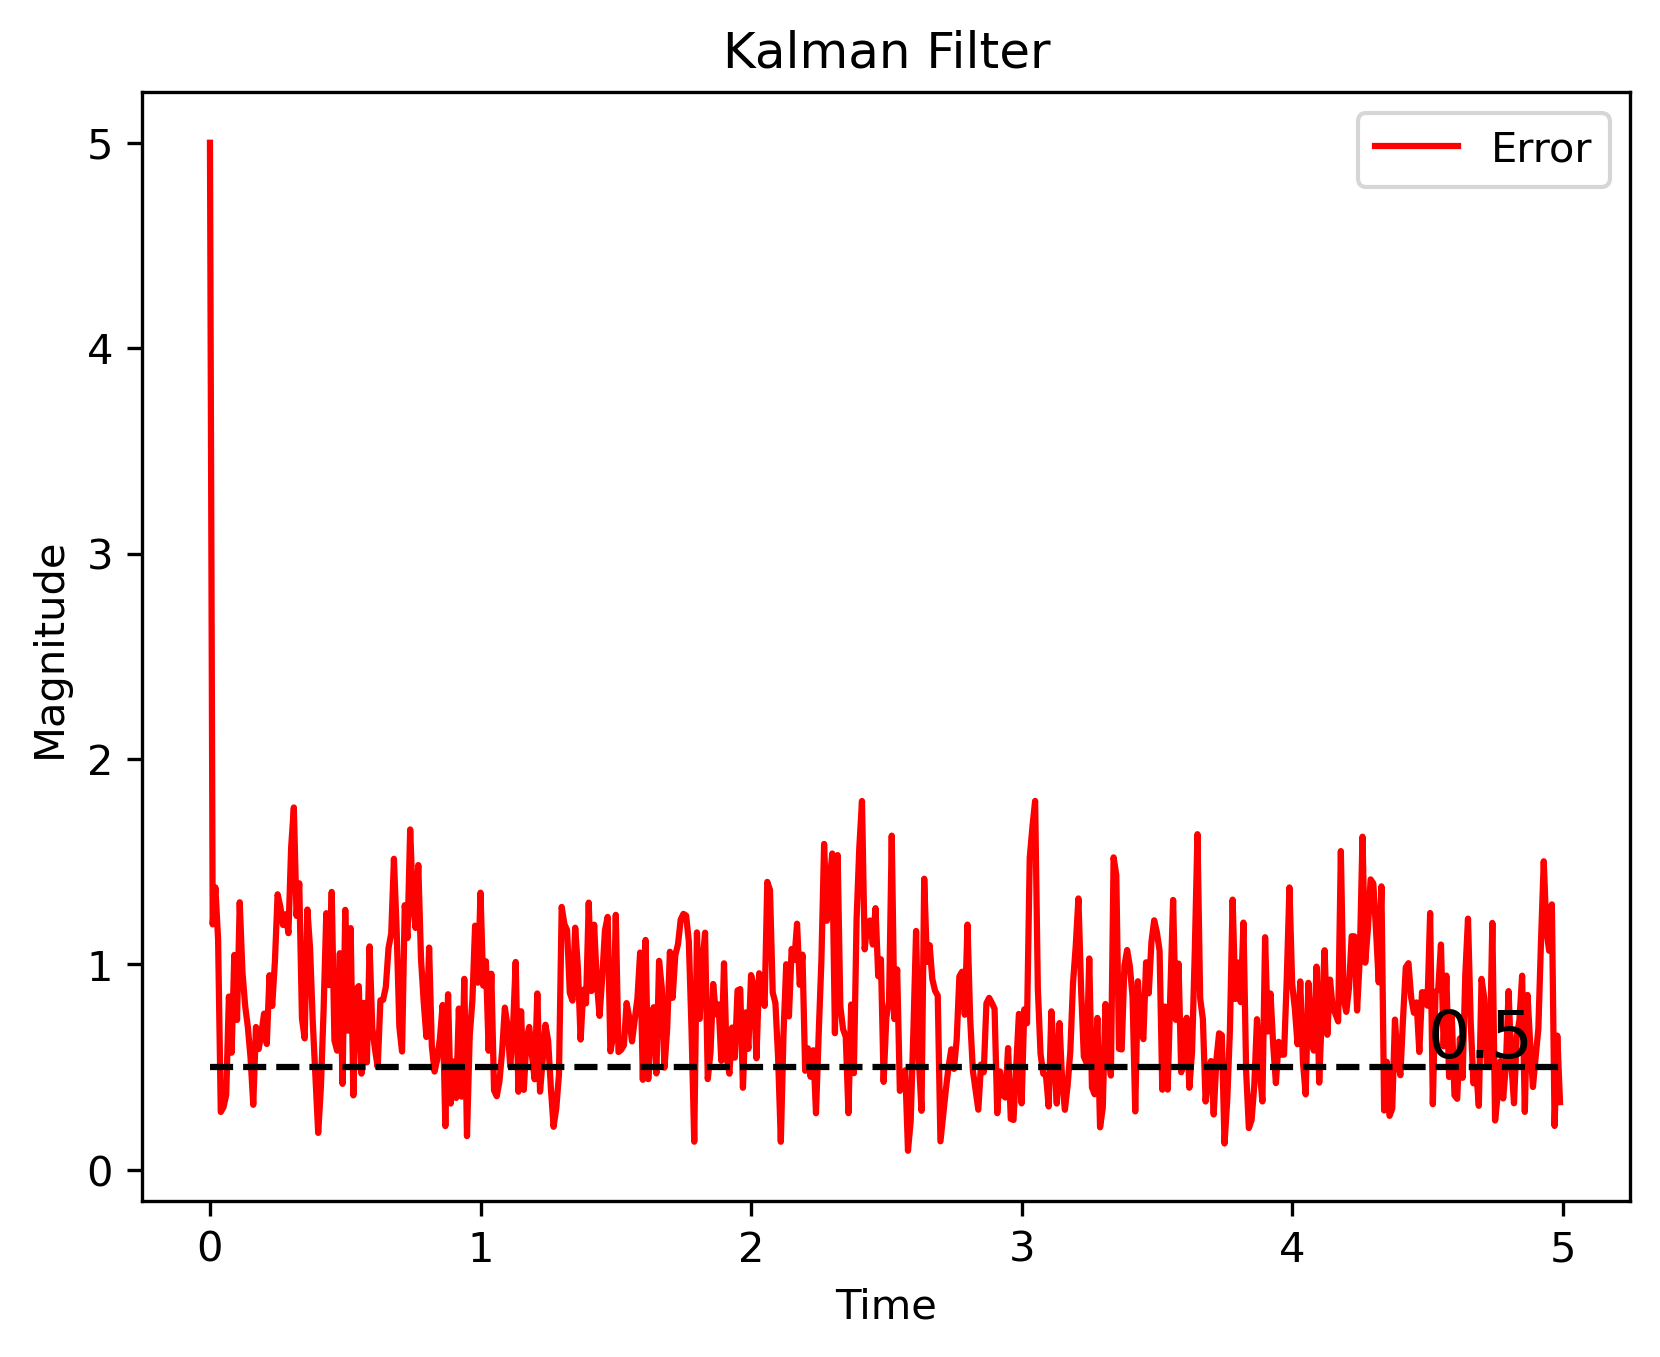
\includegraphics[width=0.75\linewidth]{graphics/Kalman3.png}
    \caption{The evolution of the root-mean-squared error in the Lorenz-63 Model with a Kalman Filter DA system.}
    \label{fig:kalman3}
\end{figure}
From Figure \ref{fig:kalman3}, we can see that the error quickly diminishes at just the beginning of DA and successfully remains at a low level that is slightly above the given observation error.

\section{Exercise}

\begin{Exercise}
Prove the following vector calculus identities using the Index Notation.
\begin{enumerate}[label=(\alph*)]
    \item $\nabla \cdot (\nabla \times \vec{v}) = 0$;
    \item $\nabla \times \nabla u = \textbf{0}$;
    \item $\nabla \times (\nabla \times \vec{v}) = \nabla (\nabla \cdot \vec{v}) - \nabla^2 \vec{v}$
    \item $\nabla \cdot (\vec{u} \times \vec{v}) = \vec{v} \cdot (\nabla \times \vec{u}) - \vec{u} \cdot (\nabla \times \vec{v})$.
\end{enumerate}
\end{Exercise}

\begin{Exercise}
Confirm that if $\vec{u}$ and $\vec{v}$ are two vectors in the tensor sense, then the cross product
\begin{align*}
w_i = \epsilon_{ijk}u_jv_k
\end{align*}
as in (\ref{eqn:crosstens}) must also be the components of a vector via Quotient Law.
\end{Exercise}

\begin{Exercise}
Given a two-dimensional plane stress with two measurements of normal/shear tractions $(7,4)$ and $(9,-3)$ that are assumed to be accurate, find the corresponding Mohr's Circle and the angle between the two oriented surfaces on which the measurements are taken.
\end{Exercise}

\begin{Exercise}
A three-dimensional stress tensor is known to have principal stresses of $\sigma_1, \sigma_2, \sigma_3 = 3,2,-1$. Determine if the following normal/shear traction pairs are possible:
\begin{enumerate}[label=(\alph*)]
    \item $(0,1)$;
    \item $(1.5,1.25)$;
    \item $(4,1)$;
    \item $(2.4,-0.6)$.
\end{enumerate}
\end{Exercise}

\begin{Exercise}
Derive the continuity equation for any extensive quantity, let's say specific humidity $q$:
\begin{align*}
\frac{\partial (\rho q)}{\partial t} + \nabla \cdot(\rho q \textbf{v}) = 0
\end{align*}
if there is no sink or source so that $dq/dt=0$.
\end{Exercise}

\begin{Exercise}
Modify the DA system in Section \ref{subsection:DAsystem} so that it only assimilates selected but not all variables (let's say, $X$ and $Z$), and also try to change the values of $R$ and $Q$.
\end{Exercise}